%        File: VTthesis_template.tex
%     Created: Thu Mar 24 11:00 AM 2016 EDT
%     Last Change: Mon, April 30, 2018
%      Author: Alan M. Lattimer, VT
%	   With modifications by Carrie Cross, Robert Browder, and LianTze Lim. 
%
% This template is designed to operate with XeLaTeX.
%
% All elements in the Title, Abstract, and Keywords MUST be formatted as text and NOT as math.
%
%Further instructions for using this template are embedded in the document. Additionally, there are comments at the end of the file that give suggestions on writing your thesis.  
%
%In addition to the standard formatting options, the following options are defined for the VTthesis class: proposal, prelim, doublespace, draft. 

\documentclass[nopageskip]{VTthesis} % nopageskip = Removes arbitrary blank pages.

% Using the following header instead will create a draft copy of your thesis
%\documentclass[doublespace,draft]{VTthesis}

% The lipsum package is just included to put dummy text in the document in order to demonstrate page headers and table of contents behavior. You should remove it once you begin writing your actual thesis or dissertation.
\usepackage{lipsum}
\usepackage{shortvrb,wrapfig,enumitem}
\usepackage{array, adjustbox, tabularx}
\MakeShortVerb{\|}
\newcommand{\ssrgContribution}{\footnote{This contribution was a shared effort with Dr. Ruslan Nikolaev, SSRG, Virginia Tech~\cite{Adelie}.}}
\newcommand{\ssrgEvolution}{\footnote{An effort to improve and extend this contribution further is ongoing by SSRG, Virginia Tech~\cite{Adelie}.}}

% Title of your thesis
\title{Linux Kernel Module Continuous Address Space Re-Randomization}

% You should include 3-5 keywords, separated by commas
\keywords{Operating systems, security}

% Your name, including middle initial(s)
\author{Muhammad Hassan Nadeem}

% Change this to your program, e.g. Physics, Civil Engineering, etc.
\program{Computer Science and Application} 

% Change this to your degree, e.g. Master of Science, Master of Art, etc.
\degree{Master of Science} 

% This should be your defense date:
\submitdate{Jan 31, 2020} 

\principaladvisor{Binoy Ravindran}
\firstreader{Ruslan Nikolaev}
\secondreader{Matthew Hicks}
\thirdreader{Danfeng (Daphne) Yao}

% The dedication and acknowledgement pages are optional. Comment them out to remove them.
\dedication{This thesis is dedicated to my parents.}
\acknowledge{This thesis came to fruition thanks to the support and advice of many people, here I would like to mention some of them:

Dr. Binoy Ravindran, my advisor, for taking me in his research group and providing me with the opportunity to work with amazingly talented colleagues. I would like to thank Dr. Binoy for his valuable guidance that shaped this thesis.

Dr. Ruslan Nikolaev, for working very closely with me every step of the way. This thesis would not have been possible without Ruslan's hands-on involvement in this project. I am grateful for all the times he spent in debugging sessions with me.

I would like to thank my committee members Dr. Hicks and Dr. Yao for agreeing to be on my committee. Thanks for taking the time to review and provide feedback on my thesis. 

My fellow researchers in Systems Software Research Group who kept me company through the thick and thin of research work and were ever willing to provide help and advice.

Finally, I would like to thank my parents. I would not have made this far if it were not for their dedication towards my education.}

% The abstract is required and should be <=250 words for thesis, <=350 words for dissertation.
\abstract{Address space layout randomization (ASLR) is a technique employed to prevent exploitation of memory corruption vulnerabilities in user-space programs. While this technique is widely studied, its kernel space counterpart known as kernel address space layout randomization (KASLR) has received less attention in the research community. KASLR, as it is implemented today is limited in entropy of randomization. Specifically, the kernel image and its modules can only be randomized within a narrow 1GB range. 
%~\cite{elixir_kernel_range:online}. 
Moreover, KASLR does not protect against memory disclosure vulnerabilities, the presence of which reduces or completely eliminates the benefits of KASLR.

In this thesis, we make two major contributions.
First, we add support for position-independent kernel modules to Linux so that the modules can be placed anywhere in the 64-bit virtual address space and at any distance apart from each other.\ssrgContribution~Second, we enable continuous KASLR re-randomization for Linux kernel modules by leveraging the position-independent model.\ssrgEvolution~Both contributions increase the entropy and reduce the chance of successful ROP attacks. Since prior art tackles only user-space programs, we also solve a number of challenges unique to the kernel code.

Our experimental evaluation shows that the overhead of position-independent code is very low. Likewise, the cost of re-randomization is also small even at very high re-randomization frequencies.

\vspace*{\fill}
This research is based upon work supported by the Office of the Director of National Intelligence (ODNI), Intelligence Advanced Research Projects Activity (IARPA). The views and conclusions contained herein are those of the authors and should not be interpreted as necessarily representing the official policies or endorsements, either expressed or implied, of the ODNI, IARPA, or the U.S. Government. The U.S. Government is authorized to reproduce and distribute reprints for Governmental purposes notwithstanding any copyright annotation thereon.

This research is also based upon work supported by the Office of Naval Research (ONR) under grants N00014-16-1-2104, N00014-16-1-2711, and N00014-18-1-2022.}

% The general audience abstract is required. There are currently no word limits.
\abstractgenaud{Address space layout randomization (ASLR) is a computer security technique used to prevent attacks that exploit memory disclosure and corruption vulnerabilities. ASLR works by randomly arranging the locations of key areas of a process such as the stack, heap, shared libraries and base address of the executable in the address space. This prevents an attacker from jumping to vulnerable code in memory and thus making it hard to launch control flow hijacking and code reuse attacks. ASLR makes it impossible for the attacker to leverage return-oriented programming (ROP) by pre-computing the location of code gadgets. Unfortunately, ASLR can be defeated by using memory disclosure vulnerabilities to unravel static randomization in an attack known as Just-In-Time ROP (JIT-ROP) attack.

There exist techniques that extend the idea of ASLR by continually re-randomizing the program at run-time. With re-randomization, any leaked memory location is quickly obsoleted by rapidly and continuously rearranging memory. If the period of re-randomization is kept shorter than the time it takes for an attacker to create and launch their attack, then JIT-ROP attacks can be prevented.

Unfortunately, there exists no continuous re-randomization implementation for the Linux kernel. To make matters worse, the ASLR implementation for the Linux kernel (KASLR) is limited. Specifically, for x86-64 CPUs, due to architectural restrictions, the Linux kernel is loaded in a narrow 1GB region of the memory.
%~\cite{elixir_kernel_range:online}. 
Likewise, all the kernel modules are loaded within the 1GB range of the kernel image.
%~\cite{elixir_kernel_range:online}. 
Due to this relatively low entropy, the Linux kernel is vulnerable to brute-force ROP attacks.

In this thesis, we make two major contributions.
First, we add support for position-independent kernel modules to Linux so that the modules can be placed anywhere in the 64-bit virtual address space and at any distance apart from each other.\ssrgContribution~Second, we enable continuous KASLR re-randomization for Linux kernel modules by leveraging the position-independent model.\ssrgEvolution~Both contributions increase the entropy and reduce the chance of successful ROP attacks. Since prior art tackles only user-space programs, we also solve a number of challenges unique to the kernel code.

We demonstrate the mechanism and the generality of our proposed re-randomization technique using several different, widely used device drivers, compiled as re-randomizable modules. Our experimental evaluation shows that the overhead of position-independent code is very low. Likewise, the cost of re-randomization is also small even at very high re-randomization frequencies.}

\begin{document}
% The following lines set up the front matter of your thesis or dissertation and is required to ensure proper formatting per the VT ETD standards. 
  \frontmatter
  \maketitle
  \tableofcontents

% The list of figures and tables are now optional per the official ETD standards.  Unless you have a very good reason for removing them, you should leave these lists in the document. Comment them out to remove them.
	\listoffigures
	\listoftables

% The following sets up the document for the main part of the thesis or dissertation. Do not comment out or remove this line.
	\mainmatter

	\chapter{Introduction} \label{ch:introduction}
        
In the earlier days of computing, an attacker could exploit a stack overflow vulnerability fairly easily to take control of the system. For example, an attacker could inject code into a program and deliberately cause a stack overflow to hijack the control flow. This kind of attack is known as a \textit{stack smashing attack} and is one of the oldest and most important exploits used to gain unauthorized access to a system~\cite{pincus2004beyond, PhrackMa67:online}. 

With the advent of \textit{Data Execution Prevention (DEP)}, code injection attacks are no longer possible. However, in spite of security mechanisms such as DEP, programs remain vulnerable to code reuse attacks. In a code reuse attack, an attacker, instead of injecting new code into the memory, now finds code fragments already existing in the program to form an exploit~\cite{Shacham:2007:GIF:1315245.1315313}. Such code fragments are referred to as gadgets. By carefully selecting gadgets, the attacker is able to perform arbitrary actions. These types of attacks, generically called code-reuse attacks, are non-trivial to defend against since the code must be executable for the program to function; nonetheless, out of order execution of code must be prevented.

Code reuse attacks are exemplified by return-oriented programming (ROP). In ROP, the attacker targets a specific program or library. The attacker uses tools such as Ropper~\cite{schirra_2019} to inspect the targeted binary and build an ROP chain to serve their malicious purpose. A ROP chain is a list of gadgets with each ending in a return statement. To perform a ROP attack, an attacker injects the stack with the list of pre-generated code pointers that each point to a gadget. After a gadget finishes execution, the return statement pops the address of the next gadget from the stack into the instruction pointer. This way, the attacker is able to piece together different fragments of code to perform arbitrary actions.

One popular mitigation against code reuse is \textit{Address Space Layout Randomization (ASLR)}~\cite{ASLR,PAXASLR}.
In ASLR, the layout of the program is randomized at load time. With the program layout randomized, each time it is loaded in memory, a traditional ROP attack comprising of pre-computed gadgets is no longer effective. In principle, all code reuse attacks can be prevented by denying the attacker knowledge of the location of code in memory. Unfortunately, an abundance of memory disclosure vulnerabilities makes it possible to defeat ASLR~\cite{cvedetails:online,strackx2009breaking}. In a Just-Tn-Time (JIT) ROP attack, with the help of these vulnerabilities, code pointer leakages can be used to unravel ASLR~\cite{JITROP,ahmed2019methodologies}.


As the sophistication of security attacks and countermeasures grow for user space programs, an operating system kernel experiences a similar increase in the number of attackers. There is an increasing number of kernel vulnerabilities that are discovered in the code of widely deployed commodity operating systems~\cite{LINUXVULN,WINDOWSVULN,MACOSVULN}. Some of the recently discovered Linux vulnerabilities such as CVE-2018-14634 are very serious and seem to have existed for over a decade~\cite{LINUXVULNDECADE}. Vulnerabilities are even more likely to be present in Linux device drivers since they are typically less tested than core kernel components, as each installation uses only a subset of drivers~\cite{cvedetails_kernel}.

There are several reasons why operating system (OS) kernels are attractive to attackers. First and foremost, defense against attacks is typically more challenging in the kernel space, which includes low-level code involving system calls, device drivers, and interrupt handlers. Second, defense mechanisms for kernel space vulnerabilities (and their inclusion in commodity OSes) often lag behind their user space counterparts. A case in point: the Linux kernel limits kernel address space layout randomization (KASLR)~\cite{KASLRLINUX},
a well-known technique against control-flow attacks, to a paltry $1$GB range on x86-64 machines due to architectural limits on instruction immediate operands~\cite{X86ABI,elixir_kernel_range:online}. Exacerbating the problem, an attacker can assume that certain memory addresses are page-aligned, which makes even unsophisticated brute-force attacks feasible.

Furthermore, OS kernel code, especially that of typical OSes in widespread production-use such as Linux, is large and complex. On the one hand, this complicates the design and implementation of defense mechanisms~\cite{ASRMINIX}. One the other hand, it gives
great flexibility for an attacker. In fact, there is a great reward
for an attacker: tampering with the kernel and gaining control of the entire system effectively enables the attacker to bypass many defense mechanisms that are deployed in user space to protect programs.

While there has been significant work done for defense against JIT-RIP and other code reuse attacks in the user space~\cite{SHUFFLER,MEMORYEXPLOIT,Wartell:2012:BSS:2382196.2382216,TASR,lu2016make,chen2017you}, research on kernel space defenses has unfortunately lagged behind. An example of defense for user space is \textit{Shuffler}~\cite{SHUFFLER}. Shuffler operates by continuously randomizing the code of a running process. By denying the knowledge of code location and continuously obsoleting memory leakages, successful formation of JIT-ROP gadgets can be prevented.

This thesis presents a defense mechanism against code-reuse attacks for kernel space, specifically targeting Linux.
Our technique contributes to Linux security in two uniquely distinguishing ways. First, the thesis extends KASLR to 64-bit address range efficiently by using the position-independent code model. Second, the thesis implements continuous re-randomization for kernel modules, an effective technique against just-in-time ROP attacks~\cite{JITROP}. Our technique is specifically designed for kernel space re-randomization and addresses the unique challenges that must be overcome to accomplish it. Unlike prior approaches for continuous re-randomization in user space~\cite{SHUFFLER}, we use a zero-copying method for moving code (and most static data as well). In addition, we efficiently keep track of, and unmap previously used address ranges.

We implement our techniques in the Linux kernel and experimentally evaluate our position-independent code support using \textit{Sysbench}~\cite{web:sysbench} and \textit{Kernbench}~\cite{web:kernbench} benchmarks as well as custom microbenchmarks. We also evaluate the cost of re-randomization for several different device drivers using microbenchmarks and real-life server applications such as Apache and mySQL. Our results reveal very little ($<$ 2\%) overhead for re-randomization compared to vanilla Linux and completely negligible overhead for supporting extended KASLR with position-independent modules.

\section{Thesis Contributions}
The thesis makes the following contributions:
\begin{enumerate}
  \item The thesis extends the range of address space layout randomization. We compile Linux kernel modules using a position-independent model that removes the prior limitation of modules having to be placed within a narrow 1GB region near the core kernel. We have compiled over 5000 modules in Ubuntu 18.04 for our testing. This contribution has already been submitted to one of the Linux kernel mailing lists as a patch, which is currently under review~\ssrgContribution~\cite{pie_patch_2:online, pie_patch_1:online}.
  \item The thesis implements a mechanism for continuous re-randomization of Linux kernel modules.\ssrgEvolution~This work, to the best of our knowledge, is the first working implementation of continuous re-randomization for the Linux kernel.
  \item The thesis demonstrates the practicality of our re-randomization approach. Our experimental studies involving stress-testing popular network and storage drivers show negligible performance impact and robustness of our re-randomization technique.
\end{enumerate}

\section{Thesis Organization}
The remainder of this thesis is organized as follows:
\begin{itemize}
    \item Chapter~\ref{ch:background} provides a background of control-flow attacks and their defenses. The chapter also presents the prerequisite base knowledge for understanding the thesis.
    \item Chapter~\ref{ch:related-word} presents prior work for preventing code reuse attacks on both user-space programs and operating systems.
    \item Chapter~\ref{ch:pic} presents the design and implementation of \textit{position-independent modules}, the first major contribution of the thesis. 
    \item Chapter~\ref{ch:re_randomization} presents the design and implementation of our \textit{re-randomization} technique, the second major contribution of the thesis.
    \item Chapter~\ref{ch:evaluation} experimentally evaluates the techniques presented in the thesis on the basis of their performance, scalability, and security.
    \item Chapter~\ref{ch:conclusion} concludes the thesis by presenting the key insights and discusses avenues for future work.
\end{itemize}
	\chapter{Background} \label{ch:background}
	    In this chapter, we discuss background information on the control-flow attacks and possible remedies against them. We also provide background information on specifics of ELF binaries in the context of position-independent code. Finally, we touch upon the Spectre vulnerability and how it affected the design of our re-randomization technique.


\section{Return-Oriented Programming (ROP)}
\label{sec:bg_rop}
\subsection{Stack Smashing Attack}

A \textit{buffer overflow} occurs when the data being written to a buffer overflows its boundaries and overwrites adjacent memory locations. A buffer overflow bug can be exploited by an attacker to manipulate the program to their advantage in what is known as a \textit{buffer overflow attack}.
A typical example of code vulnerable to buffer overflow attacks is described in Listing~\ref{lst:buffer_overflow}. The program takes a string from the command line and copies it to a local variable |buffer| in the function |foo|. A C library function |strcpy|, which is used for copying strings, just blindly copies the source into destination until a null terminator is reached.

\lstset{language=C}
\begin{lstlisting}[frame=single, caption={Buffer Overflow Example Code},label={lst:buffer_overflow}]
#include <string.h>

void foo(char *str){
    char b[8];
    strcpy(b, str);
}

int main(int argc, char **argv){
   foo(argv[1]);
   return 0;
}
\end{lstlisting}

The code in Listing~\ref{lst:buffer_overflow} works as expected for input strings of 7 characters or less (1 byte is used to store the null terminator to indicate the end of the string). A scenario when the string |HELLO| is passed to the function is illustrated in Figure~\ref{fig:stack_overflow_1}. The string including the null terminator is copied to the memory location |b[0]| to |b[5]|. The string passed is written within the confines of the buffer and the program behaves as intended.

\begin{figure}[ht!]
\centering
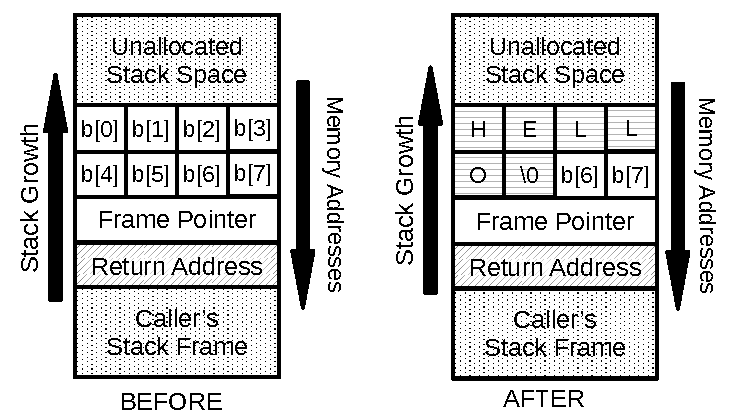
\includegraphics[width=0.7\columnwidth]{pictures/stack_overflow_1.pdf}
\caption{Snapshot of the stack before and after strcpy is called with safe input}
\label{fig:stack_overflow_1}
\end{figure}

When the function |foo| is called with an argument larger than 7 characters, the |strcpy| function overwrites the local variables defined in |foo|, the frame pointer and, most importantly, also the return address. When the |foo| function returns, the now compromised return address is loaded into the program counter and the control flow jumps to a new location instead of back to |main|. This situation is shown in Figure~\ref{fig:stack_overflow_2}. Here the command line input is ``AAAAAAAAAAAA\x02\x46\xA0\x88'', where ``AAAAAAAAAAAA'' is the code the attacker wants to execute and ``\x02\x46\xA0\x88'' is the little endian representation of the address of the local variable |b[8]| (the location in memory that contains the injected code). Note that in an actual attack, the attacker will likely put shellcode in the buffer and this way when the function |foo| returns, the shellcode would be executed, a shell would be launched and the attacker would have to ability to launch any arbitrary program.

\begin{figure}[ht!]
\centering
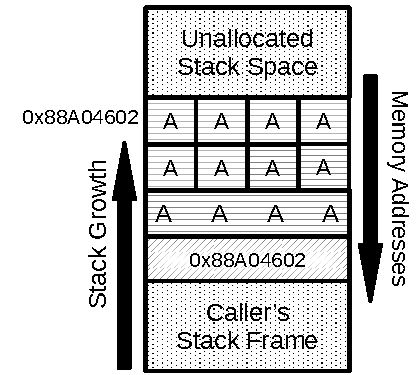
\includegraphics[width=0.35\columnwidth]{pictures/stack_overflow_2.pdf}
\caption{Snapshot of the stack after strcpy is called with unsafe input}
\label{fig:stack_overflow_2}
\end{figure}

Over the years various schemes have been developed to prevent this kind of attack. The most popular technique is data execution prevention. This technique uses a feature in modern CPUs called the Write-XOR-Execute ($W\oplus X$), also known as the NX (No-Execute) bit in x86-64 ~\cite{NXLINUX}. This feature allows memory regions to be marked as non-executable, i.e., any attempt to execute code from these regions would be prevented and an exception would be generated. The idea here is to keep all regions in memory either executable or writable but never both. Since modern operating systems mark all data pages as NX~\cite{UBUNTUNX}, this form of attack is no longer possible.

\subsection{Return-to-libc Attack}
After code injection attacks were effectively foiled by data execution prevention, a new genre of attacks known as code reuse attacks came into existence. One such attack is a return-to-libc attack. In this attack, the malicious entity does not inject code into the stack, but instead, an attacker pivots the stack to a carefully crafted call stack in memory. This way the attacker can chain the executions of a set of |libc| functions and orchestrate desired malicious behavior~\cite{nergal}. This attack goes around NX protection because the code is never executed from the stack itself but from the already existing libc code.

\subsection{Return-Oriented Programming}
Return oriented programming is a more generalized variant of the return-to-libc attack. In this technique, an attacker diverts the program control flow, but instead of jumping to a library function, a carefully chosen machine instruction already present in the code is executed. These machine instructions are called ``gadgets''. Each gadget typically ends with a return instruction. After a gadget is executed, a return address is popped from the stack into the program counter; this address is the address of the next gadget. Thus by crafting a call stack, the attacker is able to chain arbitrary machine instructions together to achieve the desired behavior. 

Figure~\ref{fig:rop_ex} illustrates how an ROP attack works. In the example, the attacker has injected three return addresses onto the stack, each pointed to a code gadget. When the original function returns, the |return address 1| is popped from the stack and the program jumps to gadget 1. When gadget 1 returns, the program jumps to the next injected return address (|return address 2|). One by one all the gadgets are executed causing the CPU to perform arbitrary actions.

\begin{figure}[ht!]
\centering
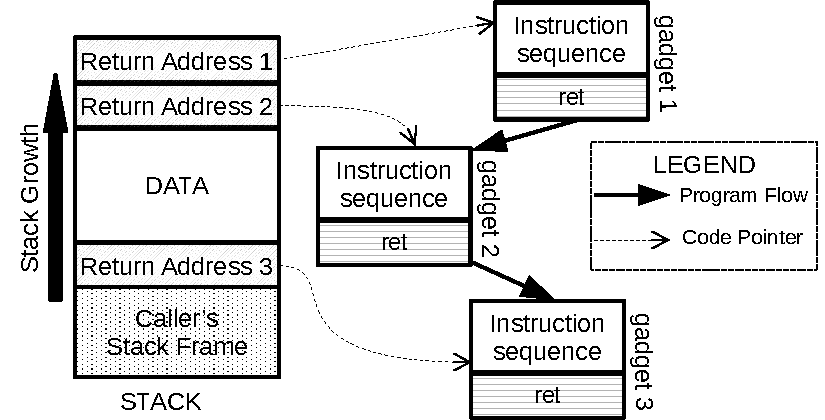
\includegraphics[width=0.65\columnwidth]{pictures/rop-min.pdf}
\caption{ROP illustration}
\label{fig:rop_ex}
\end{figure}

ROP's fundamental premise is that, given a large enough set of already loaded instructions, one can piece together a sequence of instructions that is  valid on a given ISA and accomplishes the desired malicious goal. The high density of ISAs, in particular ISAs such as x86-64, make the task of finding such a sequence of bytes or instructions easier. 

ROP is Turing-complete~\cite{Buchanan:2008:GIG:1455770.1455776}, meaning, given a sufficiently large program binary, any desired functionality can be emulated by chaining a sufficient number of gadgets. Several tools have recently been developed that can automatically create ROP payloads from program
binaries~\cite{ROPCOMPILER} -- e.g., the ROPgadget tool~\cite{ropgadget} can create an attack payload that spawns a shell that can accept arbitrary commands from an attacker.


\section{Supporting ASLR}
\label{sec:bg:aslr}
ASLR (address space layout randomization) is a widely adopted technique used to prevent exploitation of memory corrupting vulnerabilities such as stack smashing attacks. Before the advent of ASLR, operating systems would simply load an executable at a fixed address in virtual memory. With ASLR enabled, an executable or a shared library could be loaded at any random address.
At compilation time, the linker is unaware of where the code/data might be loaded, this means that the code can not directly reference other code or data in memory. In this section we discuss the two main approaches to solve this problem in Linux.

\subsubsection*{Load-Time Relocation}
A relatively straight forward way of solving this problem is to perform a load-time relocation. In load-time relocation, all the code/data references in a program are patched by the |dynamic loader| when the load address of the program is determined.

Load-time relocation has two fundamental problems.
First, it takes time to perform relocations. A complex software may reference a large number of libraries, patching each of these libraries at start-up could cause significant delays in program launch time.
Secondly, load-time relocation inhibits sharing of library code. %especially in x64 architectures. Thanks to variable/function addressing in x64 unless each program loads the library at the exact same virtual address, sharing of library code is not possible.
Loading the library at the same address is a security concern and defeats the purpose of ASLR. Therefore, the library would have to be loaded again in memory for each process that needs it. Since saving RAM is one of the most important points of having a library, using this approach is out of the question.

\subsubsection*{Position-Independent Code (PIC)}
\label{sec:bg:pic}
PIC relies on two key ideas, i.e. relative addressing and indirection. Firstly even though the program when loaded at a random address would not be able directly reference code/data, the relative offsets between code and data sections remain the same. The linker is aware of all the sections and their respective sizes at compile time and can generate code that can reference parts of the program using this already known offset. Such code uses the ``RIP-relative'' addressing mode~\cite{INTEL,AMD} in x86-64, where 32-bit offsets are added to the instruction pointer, effectively allowing the program to execute anywhere in the 64-bit virtual address space.

Most programs use dynamically linked shared libraries. Using the aforementioned RIP-relative addressing is not a suitable approach to reference a shared library because the position of the shared library relative to a program load location is arbitrary and unknown. Hence PIC adds an additional level of indirection to all library references (for both data and function calls). This indirection is implemented using Global Offset Table (GOT), discussed in Section~\ref{sec:background_got}, and Procedure Linkage Table (PLT), discussed in Section~\ref{sec:background_plt}.

The PIC model first advocated in~\cite{LIBCRET} provides support for ASLR without the limitations of Load-Time Relocation and is steadily gaining increasing popularity in Linux distributions~\cite{UBUNTUPIE} for protecting user space programs.

\subsubsection*{PIC Support in the Linux Kernel}
Both the Linux kernel and its modules as of today do not employ the position-independent model. 
There have been some preliminary efforts~\cite{LINUXPIE} to add support for position independent executable (PIE) to the Linux kernel. These efforts, however, only address the code kernel image and fail to address kernel modules.
Because of the lack of PIC support for modules,~\cite{LINUXPIE} currently extends the KASLR range from 1GB to 3GB only, which does not make a significant practical difference.
Moreover, most of the code nowadays is compiled outside of the kernel image, e.g., Ubuntu 18.04's kernel has over 5000 modules.

Our work adds support for position-independent modules in the Linux kernel. This work, thus, complements the existing PIE patch so that the entire 64-bit range can be used for KASLR. Moreover, our design enables the kernel and the modules to lie any distance apart from each other, i.e., they do not necessarily need to be placed within $\pm 2$GB range of each other.

\section{Global Offset Table (GOT)} \label{sec:background_got}
Addresses of global variables coming from a shared library are unknown, and these variables can not be accessed via relative addressing. PIC uses a level of indirection facilitated by GOT to access these variables.

GOT is simply a table (implemented as a data section in ELF) that contains the absolute addresses of all the global variables. An instruction in code that wants to reference a global variable would get the absolute address of the variable from GOT. A corresponding GOT entry retains the absolute address of the variable. The GOT entry itself is accessed like any other local variable using PC relative addressing. Consider the listings below showing a simple code example of GOT access.
\lstset{language=C}
\begin{lstlisting}[frame=single, caption={A simple C instruction that returns a variable}]
return var;
\end{lstlisting}

\lstset{language=[x64]Assembler}
\begin{lstlisting}[frame=single, caption={Assembly Code, accessing a variable using PC relative addressing}]
; access var using relative addressing and place its value in eax
mov    0x2ff6(%rip),%eax
\end{lstlisting}

\lstset{language=[x64]Assembler}
\begin{lstlisting}[frame=single, caption={Assembly Code, accessing a global variable through GOT}]
; load the address of var from GOT into rax
mov    0x5ff5(%rip),%rax
; access var and place its value in eax
mov    (%rax),%eax
\end{lstlisting}

We found GOT to be particularly useful for continuous re\hyp{}randomization.
Although the kernel uses a single address space, and shared libraries do not have the direct use in the kernel, we still want to efficiently support multiple mappings to the same code due to the ongoing re\hyp{}randomization.
GOT provides an efficient way to do so without modifying the underlying code. Although not directly provisioned by ELF shared libraries, we create multiple GOTs for different purposes within the same module to facilitate continuous re\hyp{}randomization. Specifically, using GOT for re-randomization provides us with the following benefits:

\begin{itemize}
    \item In the absence of GOT, there would be a relocation entry in the ELF file for each variable reference. These relocation needs to be patched when a module is loaded and updated when the module is re-randomized. Whereas if GOT is used, there is a need for just one relocation per variable. Generally, there are multiple references to a variable so using GOT greatly reduces the number of relocation entries. Using GOT has an added benefit during the re-randomization process as we only need to update one entry in the table per a re-randomized variable.
    \item Using GOT moves the relocation entries from the code section to the data section. This has an added security benefit as we would not have to make the code writable during re-randomization to update the variable references.
\end{itemize}

\section{Procedure Linkage Table (PLT)} \label{sec:background_plt}
PLT is a special code section which consists of a set of entries -- one for each external function. Each PLT entry is a ``trampoline'' that triggers a jump to the actual implementation of the function. Whenever an external function is called, the compiler translates it to a call to its corresponding PLT entry. The code in PLT is responsible for the lazy resolution, dynamic binding and eventual call to the requested function. The address of the intended function call is retrieved from the GOT and thus each PLT has an associated GOT entry.

PLTs are mainly used in dynamic libraries to transparently interpose on exported functions (e.g., custom \textit{malloc(2)} implementations which interpose on \textit{libc}). PLT is also used for lazy binding by dynamic linker trampolines. Although PLT does not have the direct use in the Linux kernel or in the re-randomization process, we use PLT when the retpoline mitigation is required
for better code efficiency, as discussed in Section~\ref{plt_generation}.

\section{Spectre-V2 and Retpoline}
Spectre-V2 (CVE-2017-5715) is a recent attack aimed at exploiting vulnerabilities on modern processors that perform speculative execution and branch prediction~\cite{SPECTRE}. This attack affects most existing computer systems including desktops, laptops, and mobile devices~\cite{spectre_phone_computer:online}. Spectre has been verified to work on Intel, AMD, ARM and IBM processors~\cite{Meltdown53:online,spectre_ibm:online}.
Specifically, the system is vulnerable due to indirect \textsc{call} (or \textsc{jmp}) instructions. On affected CPUs, the speculative execution resulting from a branch misprediction may leave observable side effects that could reveal private data to the attackers.

Linux uses a mitigation called |retpoline| to prevent against this vulnerability~\cite{RETPOLINE}. With this mitigation enabled, all indirect calls and jumps are replaced with |CALL_NOSPEC| and |JMP_NOSPEC| macros respectively. These macros use special \textit{retpoline thunks} that perform the jump using a |ret| instruction trampoline to prevent speculative execution. This mitigation is made possible with the support of compiler~\cite{gcc_retpoline:online,llvm_retpoline:online}.

As x86-64 does not allow 64-bit offsets for direct calls, indirect calls must be used for arbitrary 64-bit addresses. Compiling a position-independent program thus increases the number of indirect calls. And since every indirect call must use retpoline, it is crucial to optimize and minimize the number of such calls. We discuss these optimizations in Section~\ref{sec:pic:optimization}
	\chapter{Related Work} \label{ch:related-word}
	    In this chapter, we present the existing defenses against code reuse attacks. The chapter is divided into three sections, one for each category of defense.

\section{Control Flow Integrity}
Control-Flow Integrity (CFI) prevents code-reuse attacks by ensuring that the control-flow of a program remains valid. CFI enforces this property by making sure that any indirect branch taken by an application is in accordance with its control flow graph. This is done by comparing the state of the program at run-time with a set of pre-computed valid states. The application is terminated if the flow of the program diverges from expectation. In addition to user-space, CFI mechanisms have also been proposed for kernels.
KCoFI is one such compiler-based technique ~\cite{Criswell:2014:KCC:2650286.2650804}. Research has shown that CFI can be defeated by a careful selection of gadgets~\cite{evans2015control, davi2014stitching}.

\section{Code Randomization}
The second category of defenses against code-reuse is code randomization. As previously discussed, ASLR prevents reuse of the code by obscuring the location of the code in memory. Coarse-grained ASLR is currently deployed in all major operating systems~\cite{Wartell:2012:BSS:2382196.2382216, ASLR}. Address space layout randomization has been widely researched and discussed in the literature from early user-space implementations~\cite{PAXASLR,MEMORYEXPLOIT} to OS-specific
approaches such as fine-grained ASR (address space randomization) in MINIX~\cite{ASRMINIX}. Similarly, (32-bit) KASLR, which randomizes the location of the kernel and its modules at boot time is being used in Linux today~\cite{KASLRLINUX}.

Although not in wide-spread use, many fine-grained randomization schemes have also been proposed that randomize at the function, basic block or the instruction level. However, both coarse-grained and fine-grained ASLR have been defeated by JIT-ROP~\cite{JITROP}. JIT-ROP discovers code at the run time by recursively reading code pages starting with a leaked code pointer and finding other pointers. It has been concluded that no load-time randomization can protect against JIT-ROP~\cite{JITROP}. Despite being defeated, ASLR is still a promising technique that works well given enough entropy of randomization and absence of memory disclosure vulnerabilities.


\section{Code Re-Randomization}
Continuous re\hyp{}randomization was previously proposed and used in various contexts.
Stabilizer~\cite{STABILIZER} uses re\hyp{}randomization to enhance performance evaluation in user space.
Fine-grained ASR for MINIX~\cite{ASRMINIX} is an early implementation of
re\hyp{}randomization for MINIX OS~\cite{MINIX}, a modular microkernel-based operating system.
Shuffler~\cite{SHUFFLER} is a user-space technique for continuous re\hyp{}randomization to protect against JIT ROP attacks.
Although we solve the same problem in kernel space that Shuffler solves in user space, Shuffler's goals are somewhat different from ours: it relies on the binary transformation of user-space programs,
whereas we propose a technique that benefits from Linux source code availability
as well as from the position-independent model as used by our modules.

There also exist (user-space) techniques that rely on compiler support. Remix~\cite{REMIX}
extends the LLVM compiler to add extra nop paddings, allowing runtime flexibility
for moving code inside functions. This way gadget locations change. However, attackers
can still use function pointers to defeat this re\hyp{}randomization scheme.
TASR~\cite{TASR} is another system based on the assumption that re\hyp{}randomization in the
program should happen before input and output (between corresponding system calls).
TASR is only suitable for user-space programs and has a very high overhead.

Other techniques aim to enhance OS security by other means. NICKLE~\cite{KERNELROOTKITS}
uses virtual machines to run kernel code in shadow regions. The kernel code can be transparently
executed in virtual machine in runtime. Similar techniques also used by HookSafe~\cite{HOOKSAFE}
and hvmHarvard~\cite{HVMHARVARD}.
Other techniques such as~\cite{KERNELCONTROLDATA} rely on
special compiler support to protect kernel control data.
Unfortunately, none of these techniques provide an exhaustive solution to security
problems that modern OSes have to deal with.

Our work also differs from existing approaches in its focus on large-scale, monolithic OS
kernels such as Linux which use a low-level programming model and have many inter-connected
components that do not have strict boundaries and are not well isolated from each other.
We also provide a comprehensive solution that can be adapted to a wide range of kernel modules.

% \section{Comparison with Shuffler}
User-space continuous re\hyp{}randomization was previously studied in Shuffler~\cite{SHUFFLER}. Although Shuffler's goals are partially aligned with ours, the objectives and challenges in both cases are not identical. Shuffler is only intended for user-space programs and does not
handle low-level code such as system calls, interrupt handlers, etc.


In-kernel code is also often written to be agnostic to threads that use it: function calls can go all the way from system calls initiated by different user programs and threads. Moreover, Shuffler benefits
from already existent rich support for position-independent code in user space. Challenges of implementing randomization and re\hyp{}randomization in OS environments were previously pointed out in~\cite{ASRMINIX}, an early attempt to solve a similar problem for more componentized microkernel-based
OS designs such as MINIX~\cite{MINIX}.

We also take a different approach to performing re\hyp{}randomization. While
Shuffler performs binary rewriting of existing binaries, we
do not use binary-level transformation. Due to source code availability
of the kernel and most of its modules, it makes more sense to
have a solution that requires a relatively small number of changes while
benefiting from source code access. Shuffler also has certain
limitations such as requiring an executable and all required libraries
to be within $\pm 2$GB reach from each other, effectively transforming
dynamically-linked applications to more monolithic, statically-linked binaries.
	\chapter{Position Independent Modules} \label{ch:pic}
	    The importance of implementing position-independent code model for Linux kernel modules was discussed in Section~\ref{sec:bg:aslr}. In this chapter, we discuss our methodology of generating GOT and PLT in order to support the PIC model for the kernel modules.

\section{Design}
A shared library comprises of multiple files of source code. In a typical compilation process, each source code file (.c file) is first compiled into an |object file| (.o file) and finally all the object files are linked together to form a |shared object| (.so file). An object file is an intermediate file that is not fully linked, it contains relocation entries and metadata to facilitate further linking. A shared library, on the other hand, is produced further in the linking process; it is largely relocated and has fully generated GOTs and PLTs.

In our implementation, we chose to load kernel modules as object files rather than shared object files. Since an object file contains relocations and meta-data for further linking, they are easier to work with. With the flexibility provided by an object file, we design our own implementations of PLTs (Section~\ref{plt_generation}) and GOTs (Section~\ref{sec:pic:got}) which are highly optimized and suitable for re-randomization.

PLT stubs are typically used in position-independent code to facilitate function interposition and lazy binding for shared libraries and have no direct use in the kernel. However, we found that the Spectre-V2 mitigation (in the presence of PIC) creates code bloat as corresponding retpoline-based calls use longer sequences of instructions, clobber registers, etc. To support retpoline more efficiently, we enable PLT stubs on Spectre-vulnerable machines when retpoline is enabled.

Depending on whether the target CPU has the Spectre-V2 mitigation enabled or not, we apply appropriate optimizations, discussed in Section~\ref{sec:pic:optimization}, to patch the code in order to minimize the need of PLT entries. After the PLTs/GOTs are generated and necessary optimizations are applied, we change the permissions of the pages to read-only to protect the memory from being exploited by an attacker.


\section{Optimizations}
\label{sec:pic:optimization}
\subsubsection*{PLT Optimizations}
As previously discussed, the retpoline mitigation causes significant differences in the code generated at the function call sites. We optimize our implementation of PIC for both of these cases -- when retpoline is enabled and when it is disabled.

When the kernel is configured with retpoline disabled, we compile the module with the \verb|no-plt| gcc flag. This causes gcc to avoid PLT. Instead of jumping to a PLT stub, the code gets the callee address from the GOT and indirectly branches to it.
Given the size of the module does not exceed 2GB, all the local functions and code pointers of the module are guaranteed to be within the range of $\pm 2$GB from the call site. In this case, indirect branches to 64-bit absolute addresses through GOT can be replaced with 32-bit PC relative direct branches. Therefore, for all local symbols indirect \verb|call/jmp| instructions are replaced with direct \verb|call/jmp| respectively. This optimization provides two benefits. First, slower indirect branches are replaced with faster direct branches.\footnote{Indirect branches are slower because they involve an extra indirection. The CPU has to read (data) memory to calculate the target address.} Second, it avoids the need for retpoline safe indirect jumps on processors vulnerable to the Spectre-V2 attack. Since direct \verb|call/jmp| instructions are 1 byte shorter than their indirect counterparts, they are padded with \verb|nop|:
\begin{verbatim}
    call *foo@GOTPCREL(%rip) --> call foo; nop
    jmp *foo@GOTPCREL(%rip)  --> jmp foo; nop
\end{verbatim}

Conversely, if the kernel is configured with retpoline enabled, we do not set the |no-plt| flag and the generated code makes branches though PLT. The PLT stubs are specially generated for safe indirect jumps that mitigate Spectre-V2 attacks. These stubs can be very expensive, so we eliminate PLT stubs for local symbols by replacing 32-bit PC relative calls to PLT stubs with 32-bit PC relative calls straight to the relevant symbols as follows:
\begin{verbatim}
    call foo@PLT --> call foo
    jmp foo@PLT --> jmp foo
\end{verbatim}

\subsubsection*{GOT Optimizations}
Similar to the optimizations made to the local function calls, local variable accesses are also optimized. When modules are compiled with PIC, compiler-generated code retrieves the address of all variables through GOT by default. Considering the small size of the kernel modules, all the local variables are guaranteed to be within $\pm 2$ GB range of the access site and can be referenced directly without going through GOT. We patch all accesses to the local variables as follows:
\begin{verbatim}
    mov foo@GOTPCREL(%rip), %reg --> lea foo(%rip), %reg
\end{verbatim}

All of the aforementioned optimizations not only provide immediate performance benefits by cutting down unnecessary indirections, they also help in reducing the number of GOT and PLT entries. Optimizations applied to local symbols substantially reduce the number of GOT entries for local symbols. Smaller GOT and PLT tables save memory and reduce the risk of leaking absolute variable addresses to an attacker. Moreover, having small GOTs is important for fast re-randomization. During re-randomization, when the code is moved to a new memory location, the GOT needs to be updated accordingly. Since most of the GOT entries are eliminated with our optimizations, a substantially smaller number of GOT entries needs to be updated, resulting in low re-randomization overhead.

\section{GOT Generation}
\label{sec:pic:got}
As previously discussed, compilers do not generate GOT for relocatable *.o object files. Since our implementation relies on GOTs, we create our own tables at module load time. Empty (i.e., 0-byte) sections for GOT are added to the object file at link-time using a custom linker script. These empty sections are then inflated to appropriate sizes by traversing over the relocation tables and counting the number of required GOT entries. Finally, the GOT is lazily populated when a relevant relocation type is encountered while the relocations are being applied. The algorithm for generating GOT is discussed in detail below.

Every symbol that has a relocation entry with any of the following relocation types requires a GOT entry:
\begin{verbatim}
R_X86_64_REX_GOTPCRELX
R_X86_64_GOTPCRELX
R_X86_64_GOTPCREL
R_X86_64_PLT32
\end{verbatim}
Each symbol is typically referenced by multiple relocation entries but requires only one GOT entry. Our solution to this problem is to sort the relocation table with respect to two keys, namely |relocation type| and |symbol|. We use Linux's (in place) heapsort function with a custom comparator for this purpose. The comparator first compares the relocation type and then the symbol. Sorting this way brings together all the relocation entries that refer to the same symbol. This method is not perfect since an object file may contain multiple relocation tables. These relocation tables are not consecutive in memory and can not be sorted together. In cases where the object file contains multiple relocation tables that have relocation entries referring to a common symbol, this algorithm would generate some duplicates. The only drawback of having duplicate GOT entries is wasted memory. An alternative to sorting would be to use a hashmap to weed out the duplicates. A hashmap requires O(number of symbols) memory. Our experiments showed that with our implementation less than 4\% of the GOT entries are duplicates. Given the simplicity of this implementation and a relatively small number of duplicates, this algorithm is found to be a good compromise.

After the size of GOT is determined by counting the number of unique symbols that require a GOT entry, it is time to populate the table. While relocations are applied, whenever a \verb|GOT| relocation type is encountered, a new entry is written into the GOT. The GOT entry contains the 64-bit absolute address of the corresponding symbol.

\section{PLT Generation} \label{plt_generation}
Similar to the generation of GOT, PLT generation also involves adding an empty section to the object file, inflating the section by counting the number of required PLT entries and lazily creating the entries when a relevant relocation entry is encountered at load time.

The number of required PLTs is calculated by counting the number of unique symbols referred to by the \verb|R_X86_64_PLT32| relocation type. Here, again, sorted relocation tables are used to filter out the duplicates. And just like with GOT, some duplicate PLT entries may be generated. Duplicate PLTs have the undesirable effect of wasting memory but they do not affect the correctness of the module. Through our experiments, it was found that \textasciitilde3\% of the PLT entries are duplicated.

While applying relocations, whenever a relocation of the \verb|R_X86_64_PLT32| type is found, a new PLT entry is generated. For each generated PLT, a new GOT entry is also created. The GOT entry contains the absolute address of the symbol referenced by the relocation entry. The PLT entry depends on the Linux configuration. If retpoline is enabled, the function address is loaded into the \verb|%rax| register from the GOT entry and a safe jump is made to \verb|%rax|.\footnote{According to the x86-64 ABI, \textsc{\%rax} is a temporary register which is not preserved across function calls. This essentially means that \textsc{\%rax} could be clobbered without backup. Even though Linux occasionally uses non-standard calling conventions, \textsc{\%rax} seemed the safest choice for a temporary register here. A few non-standard \textsc{\%rax} uses are handled separately.} Linux's \verb|JMP_NOSPEC| macro is used for the safe jump; this macro takes care of determining if the CPU is affected by the Spectre-V2 bug and generates safe and optimized code. Listing~\ref{lst:plt_retpoline} shows the generated PLT stub when the kennel is compiled with retpoline enabled.

\lstset{language=C}
\begin{lstlisting}[frame=single, caption={PLT Stub when Retpoline is Enabled},label={lst:plt_retpoline}]
movq foo@GOTPCREL(%rip), %rax
JMP_NOSPEC %rax
\end{lstlisting}

\pagebreak
Conversely, if the kernel is configured with retpoline disabled, the generated PLT stub is simply an indirect jump to the appropriate function as shown in Listing~\ref{lst:plt_no_retpoline}.

\lstset{language=C}
\begin{lstlisting}[frame=single, caption={PLT Stub when Retpoline is Disabled},label={lst:plt_no_retpoline}]
jmpq    *foo@GOTPCREL(%rip)
\end{lstlisting}
	\chapter{Re-Randomization} \label{ch:re_randomization}
	    For our initial design, we restricted the problem of re-randomization to only kernel modules. The argument here is that most of the kernel code (i.e., most of the device drivers, kernel libraries, etc) can be compiled as modules and the size of the core kernel can be reduced to the bare minimum. Possibility of JIT-ROP attacks on the core kernel can be minimized by scrutinizing the kernel code, ensuring that it is free of any memory disclosure vulnerabilities.
The kernel still uses KASLR -- the kernel image is loaded at a random address at boot time but is not re-randomized subsequently. The distribution and availability of ROP-gadgets across the kernel and its modules is analyzed in Section~\ref{se:eval_security}.

In the following sections, we describe how we implement efficient run-time re-randomization of the kernel modules. We describe how a module is logically split to aid re-randomization. The algorithm for stack and module re-randomization is also discussed in detail.

\section{Module Organization}\label{se:module_organization}
Every re-randomizable kernel module is split into two logical parts: \textit{movable} and \textit{immovable}. The movable part contains all of the code and most of the data, and the immovable part contains glue code (function wrappers) and some data (that need to be stored with the kernel). During re-randomization only the movable part of the kernel is relocated to a new address space while the immovable part remains static. Since the immovable part does not contain any module functionality and is never moved, it can be thought of as an integral part of the kernel. In Figure~\ref{fig:design}, we show a typical module layout.

\begin{figure}[ht!]
\centering
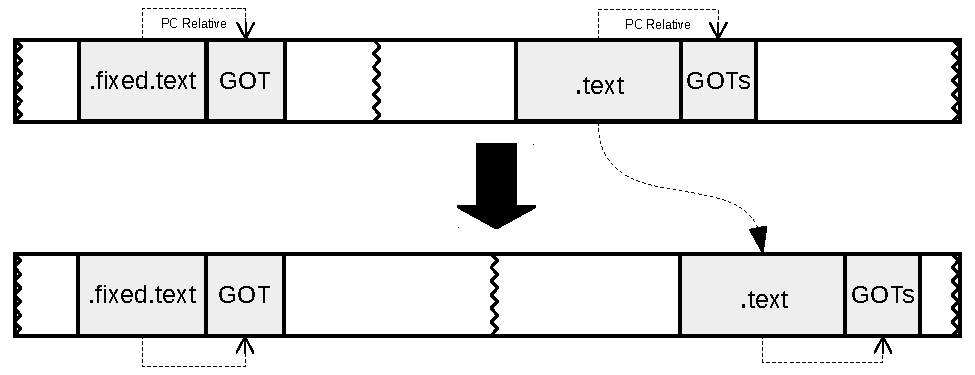
\includegraphics[width=.8\columnwidth]{pictures/rand_got.pdf}
\caption{GOT}
\label{fig:gots}
\end{figure}

\begin{figure}[ht!]
\centering
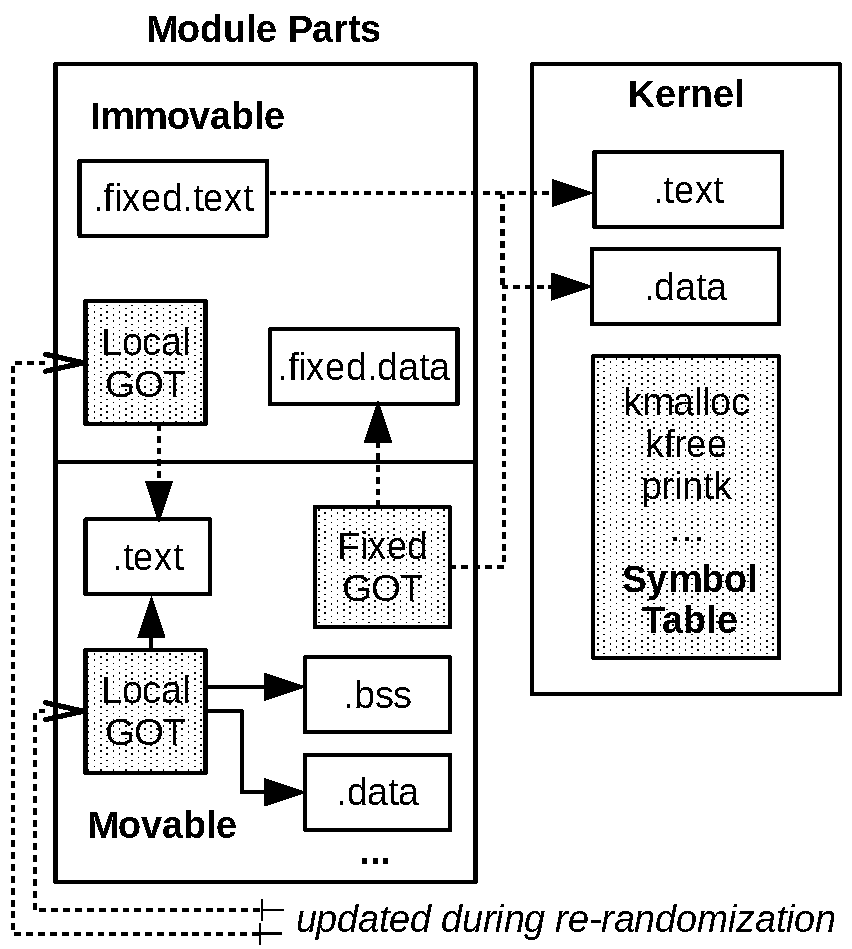
\includegraphics[width=.6\columnwidth]{pictures/design.pdf}
\caption{Design of re-randomizable modules~\cite{Adelie}}
\label{fig:design}
\end{figure}

The immovable and movable parts of the module can be placed anywhere in the 64-bit address space but due to ISA limitations, GOTs need to be within $\pm 2$GB of the code where they are accessed. This restriction arises from the fact that GOT entries are accessed using PC relative addressing which imposes a limitation on the distance between the table and the code that accesses it. This is why we need to maintain separate GOT tables for each part of the module.

A GOT table may contain two types of symbols: static and non-static (randomized) symbols. Static symbols, like global kernel references, do not need to be updated at the time of randomization while randomized symbols, like module-local symbols, are updated during randomization. To easily identify and update all the non-static symbols in the module, we create two GOTs. \textit{Fixed GOT}, that contains all the static symbols and \textit{Local GOT}, that contains all the symbols that need to be updated on re-randomization.

The movable part of the module contains both GOTs while the immovable part of the module only contains \textit{Local GOT}. As this part comprises only of thin function wrappers written entirely in assembly, the need for \textit{Fixed GOT} is avoided by directly having the 64-bit address of fixed functions in the code.

\section{Zero-copy Address Re-Map}
A major novel aspect of our work is that, unlike Shuffler~\cite{SHUFFLER}, we completely avoid copying of code and static data while re-randomizing addresses.
In Figure~\ref{fig:architecture}, we demonstrate the high-level principle.
Initially, at instant 1, both the kernel and the modules are in some randomly chosen address space, any distance apart from each other. This is achieved using our extended 64-bit KASLR. Periodically, module locations are re-randomized by a special \textit{randomizer} kernel thread. This thread creates new mappings, as shown at instant 2. Finally, when old regions are no longer used, we unmap them. In this process, no copying is actually made; we simply create a new page table entries that point to the same physical memory location.

\begin{figure}[ht!]
\centering
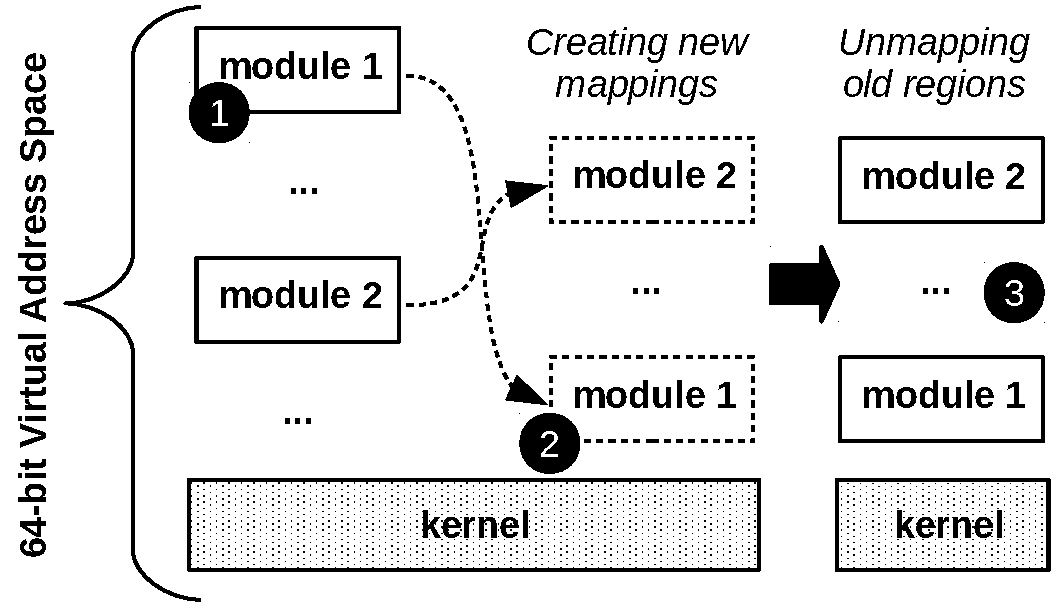
\includegraphics[width=0.7\columnwidth]{pictures/architecture.pdf}
\caption{Zero-copy mechanism~\cite{Adelie}}
\label{fig:architecture}
\end{figure}

\section{Controlling Address Space Lifetime}
It is crucial to timely delete old code from the memory, so that gadget addresses quickly become obsolete and useless for an attacker. Techniques used today (e.g., in Shuffler~\cite{SHUFFLER}) involve making a new copy of code, pausing threads, and unwinding the stacks. Previous code copy is removed after all the threads are done unwinding and updating the symbols on their corresponding stacks. While these techniques work in user space, kernel code is quite complex and functions can be called through long chains eventually leading to some user space thread making a system call. Due to low latency requirements of operating systems, the approaches that require pausing execution are infeasible and impractical to be used in the kernel space.

Our solution to this problem is to use deferred unmapping. The main idea
is to let pending calls finish execution in the old virtual address space. All function calls post re-randomization execute in a new virtual address space. Both old and new virtual address spaces map to the same physical pages, making simultaneous execution possible. As soon as the last pending call completes, the previous address range is immediately unmapped. Since almost all
kernel space calls should be relatively quick (or, otherwise it 
would indicate some bug in the code), the old pages do not stay mapped in memory long enough to be useful to an attacker.

The main challenge in effective address space lifetime management is to keep track of pending calls with little
overhead and in a scalable manner. Although the technique of reference counting~\cite{LFRC} used in memory reclamation can solve this problem, it can be slow in multi-core systems where updating a global
reference counter creates a hotspot for multiple CPUs. Instead,
we use the Hyaline lock-free memory reclamation~\cite{nikolaev2019hyaline}, which largely solves the same problem of efficient, optimistic memory access to blocks that are concurrently being deallocated by other threads. The main idea of the approach is to enclose operations that access potentially disappearing memory blocks with |mr_start()| and |mr_finish()|.
These special operations postpone memory reclamation until after all pending calls (i.e., those that
called |mr_start|) execute |mr_finish()|.
In this model, memory blocks are not de-allocated directly, instead, they are first \textit{retired} with
a special |mr_retire| operation. Only after pending calls from all threads complete, does the de-allocation take place. We refer the reader to~\cite{nikolaev2019hyaline} for more details regarding the Hyaline lock-free memory reclamation.

\section{Function Wrapping}
\label{se:function_wrapping}
One crucial step for making a module randomizable is wrapping all of its externally accessible functions. Any module functions that can be called by rest of the kernel must be wrapped for three reasons:

- First, this allows module address space to be re-randomized without breaking any function pointers that the kernel may hold. Module functions are not directly exposed to the kernel. Instead, all the external functions are wrapped with a thin wrapper, and the reference to the wrapper is passed to the kernel. By placing the wrapper function in the fixed part of the module, the movable part of the module can be freely moved in the memory whilst still maintaining valid kernel pointers. At the time of re-randomization, the function wrappers must be patched to point to the new location of the module, as discussed in detail in Section~\ref{se:module_randomization}.

One might argue against the indirection introduced by function wrappers and suggest directly updating the kernel pointers after re-randomization. This raises certain challenges. The pointer passed to kernel may propagate, in which case, all the pointers must be tracked and updated. Certainly there exist previous works on pointer tracking. However due to the Linux kernel's non-standard use of pointers\footnote{Pointers are sometimes used in kernel in non-standard ways. For example, LSB of pointers is sometimes used for a flag. Hence pointers can not be directly and automatically updated without considering the context of each individual pointer.} \cite{Linux_Pointer_NON_STD} this problem becomes intractable.

- Second, wrapping all the entry points to the module provides an easy way to control its address space lifetime using memory reclamation.

- Third, wrapping functions allows for the module's stack to be randomized. Stack randomization is discussed in Section~\ref{se:stack_randomization}.

Listing \ref{lst:before_wrapping} and \ref{lst:after_wrapping} give a high level overview of how a function wrapper works. The original function named \verb|func| is renamed to \verb|func_real| and a wrapper function with the name of \verb|func| is created that calls the actual implementation \verb|func_real|. The rest of the module keeps using the name \verb|func| in its code.

\lstset{language=C}
\begin{lstlisting}[frame=single, caption={Original Function},label={lst:before_wrapping}]
long func(long arg)
{
    // code
}

kernel_ref(&func);
\end{lstlisting}

\lstset{language=C}
\begin{lstlisting}[frame=single, caption={Wrapped Function},label={lst:after_wrapping}]
/* Movable function */
long func_real(long arg)
{
    // code
}

/* Fixed function */
long func(long arg)
{
    mr_start();
    randomize_stack();
    long ret = func_real(arg);
    restore_stack();
    mr_finish();
    return ret;
}

kernel_ref(&func);
\end{lstlisting}

\subsection{Naked Wrapper}
The function wrappers are implemented as \verb|naked| functions. A naked function is a special function for which the compiler does not generate any prologue or epilogue. These functions can only contain assembly instructions. Naked functions are used instead of pure assembly functions to take advantage of compiler type checking. Writing the wrapper function in the assembly has two advantages. Firstly, it allows for freedom of doing non-conventional things like randomizing the stack of a running program. Secondly, wrapper function could be made really thin by explicitly avoiding calls through PLT or GOT.

In x86-64, the first six arguments to a function are passed through registers. At the entry point of the wrapper, registers |rdi|, |rsi|, |rdx|, |rcx|, |r8| and |r9| contain the arguments for the wrapped function. However, before the wrapped function is called, we need to call other functions such as |mr_start()| and |randomize_stack()|. Calling these functions before the wrapped function could clobber the registers, destroying any arguments passed by the caller. Similarly, function's return value is also returned through a register. Thus the return value of the wrapped function could also be destroyed by subsequent calls to |mr_finish()| and |restore_stack()|. The registers must, therefore, be carefully handled to ensure the preservation of the arguments and return value of the wrapped function. In our implementation of the wrapper, we follow the x86-64 ABI for function calls. We push all the volatile registers containing arguments for the wrapped function onto the stack at the beginning of the wrapper. The registers are then restored before the wrapped function is called. Wrapped function's return value is also similarly saved and restored. The pseudo-code for the naked wrapper function is described in Listing~\ref{lst:naked_wrapper}.

\lstset{}
\begin{lstlisting}[frame=single, caption={Naked Wrapper Function},label={lst:naked_wrapper}]
Save base pointer
  Push arguments to the stack
    Call mr_start() and randomize_stack()
  Pop arguments from the stack
  Call wrapped_function()
  Save return value
    Call mr_finish() and restore_stack()
  Restore return value
Restore base pointer
\end{lstlisting}

\section{Data Wrapping} \label{se:data_wrapping}
Similar to function wrapping, all the structs and variables passed to the kernel must be wrapped as well. The kernel could keep a reference to any data structure passed to it. These data structures must hence be placed in the fixed part of the module. Placing them in fixed sections keeps the kernel references valid while the movable part of the modules is relocated to a new address space. Section placement is achieved  by using the \verb|section| attribute of GCC compiler. The variables are placed in the \verb|.fixed.data| section and constants are placed in \verb|.fixed.rodata|. During re-randomization, all the fixed sections are recognized by the |.fixed| prefix in their section names and are left as is.

\section{Stack Randomization}
\label{se:stack_randomization}
Randomizing stack is not a trivial task. Linux kernel maintains multiple stacks for each task. Each thread needs its own stack and the stack randomization process needs to be fast. Device drivers typically have many interrupts registered. Interrupt handlers run asynchronously, preempting other tasks and interrupt handlers. While an interrupt is being served other interrupts in the systems may also be disabled. Any delays in the top half of the interrupt service routine can have severe repercussions. Therefore it is really important to have a fast stack swapping methodology.

Our approach is to maintain a per-CPU lock-free (LIFO) list of stacks. We randomize the stack at the beginning of the function wrapper by dequeuing the head of the per-CPU list. Old \verb|%rsp| is saved in the \verb|%rbp| and \verb|%rsp| is replaced with the newly dequeued stack. Before exiting the wrapper the stack is returned to the head of the queue and \verb|%rsp| is restored from \verb|%rbp|.

The LIFO implementation of the list provides good temporal locality. High frequency interrupts grab and release the same stack, this ensures that the cache is always hot and causes minimal thrashing. Moreover, since a different list is implemented for each CPU the contention is low and high performance is achieved.

For performance reasons, the anticipated number of stacks are eagerly allocated and kept in the LIFO list. Eager allocation of stacks prevents costly \verb|kmalloc| calls in the wrapper functions. Through experiments we found that five stacks for each CPU are enough for most purposes, although in rare cases when more stacks are needed, they will be dynamically allocated as shown in Listing~\ref{lst:get_stack}.

In the head of the list we keep a \verb|version| field, this field is used to prevent the old stacks from being reused after re-randomization. At the time of randomization we create a new per-CPU list of stacks with incremented $version$. The old lists are replaced by new ones by a \verb|CAS| operation. All the elements on the old list are emptied into per-CPU \verb|trash list|. At this point, all the old stacks that are currently not checked-out are taken out of circulation. To avoid putting the old stacks back into the list, whenever a stack is returned, its \verb|version| is checked. If it does not match the \verb|version| of the list head, it is put into \verb|trash list| instead of the LIFO list. It is important to note that even though all the stacks are removed from the LIFO list, it is not safe to free them just yet. This is because a sleeping thread which is in the process of dequeuing a new stack from the LIFO list may still hold a reference to it. We have to wait till all the threads have left the address space of the module and it is safe to reclaim memory. The |trash lists| are then traversed and all the old stacks are freed.

x86-64 accepts the first six function arguments through the registers and any additional arguments are passed on the stack \cite{X86_ABI}. In our work, we did not discover any function calls with more than six arguments, so we simply replace the stack pointer to point to the new randomized stack. Any local variables passed by reference will remain on the old stack and the pointer arguments will keep pointing to them. This implementation avoids the lengthy process of stack unwinding and copying, and allows us to keep stack swapping logic minimal. All the functions executed from the untrusted module, however, will use the new randomized stack.

\lstset{language=C}
\begin{lstlisting}[frame=single, caption={Stack Randomization},label={lst:stack_randomization}]
%rbp = %rsp;
%rsp = get_stack();
...
return_stack(%rsp);
%rsp = %rbp;
\end{lstlisting}

\lstset{language=C}
\begin{lstlisting}[frame=single, caption={get\_stack()},label={lst:get_stack}]
void *get_stack()
{
    void *stack = pop_stack_this_cpu();
    if (stack == NULL)
        stack = allocate_stack();
    return stack;
}
\end{lstlisting}

\lstset{language=C}
\begin{lstlisting}[frame=single, caption={return\_stack()},label={lst:return_stack}]
void return_stack(void *stack)
{
    push_stack_this_cpu(stack);
}
\end{lstlisting}

The lock-free LIFO list implementation is standard and is not documented in this report. The only deviation from the standard is that we have used some bits of the $aba\ stamp$ word to track the $version$ and $size$ of the stack, see Listing \ref{lst:stack_head}. x86-64 only supports 128-bit compare-and-swap ($CAS$) operations, 64 bits are required to store the pointer to the head node, the remaining 64 bits are usually used to store the aba stamp. Since our head must fit in 128 bits for $CAS$ operation, in our implementation we used bit-fields to split the 64 bit word into aba, version, and size. For practical purposes, a 48-bit aba stamp is enough to solve the ``ABA problem''~\cite{CAS_Reactor}.

\lstset{language=C}
\begin{lstlisting}[frame=single, caption={Head Structure},label={lst:stack_head}]
struct head {
	struct stack_node *head;
	union {
		struct {
			u64 size:8;
			u64 ver:8;
			u64 aba:48;
		};
		u64 stamp;
	};
} __aligned(16);
\end{lstlisting}

\section{Module Re-Randomization}
\label{se:module_randomization}
The process of loading a module is different for re-randomizable and non-re-randomizable modules. Vanilla Linux allocates the module in two chunks, \textit{init} \verb|module_layout| containing the module initialization code and \textit{core} \verb|module_layout| containing the core functionality of the module. For re-randomizable modules, we create an additional \textit{fixed} \verb|module_layout| for the fixed part of the module. For a re-randomizable module, all the sections that are identified to be fixed are allocated in the \textit{fixed} layout at load time.

In vanilla Linux, once the module is done loading, all the artifacts that are no longer required are freed. Specifically, relocation and symbol tables are deallocated from the memory. However, since we need to patch the binary again each time it is randomized, we save the relocation and the symbol tables.

Reapplying relocations is a costly process, we are mindful to only keep the relocations that are required. Under the position-independent code, most of the relocations are not required to be reapplied and can be gotten rid of. We remove all the relocations of the following types:
\begin{verbatim}
R_X86_64_PC32,
R_X86_64_PC64,
R_X86_64_REX_GOTPCRELX,
R_X86_64_GOTPCRELX,
R_X86_64_GOTPCREL,
R_X86_64_PLT32
\end{verbatim}
Furthermore, we also remove the relocations of type \verb|R_X86_64_64| that reference fixed symbols.

For re-randomizable modules, we have three GOTs instead of one. Based on section (fixed vs. movable parts) and symbol locality, we choose one of those tables when generating a corresponding entry. Occasionally, two tables will contain duplicates of the same symbol (e.g., a local GOT entry
from the immovable part can point to the same address as a local GOT entry from the movable part). We use separate GOTs for movable and fixed parts because these parts can be any distance away from each other, while GOTs must always be placed within $\pm 2$GB reach from \%rip due to the ``RIP-relative'' address mode, as discussed in detail in Section~\ref{se:module_organization}.

During module re-randomization, the randomizer kernel thread periodically performs the following steps:
\begin{enumerate}
\item A new virtual address space map is created that maps to the same physical addresses as an old map. This mitigates the need of copying the module code and data.

\item The addresses of the randomized symbols in the symbol table are updated. This symbol table is subsequently used to reapply the relocations.

\item Randomized symbols in the movable GOT are updated.

\item The module is patched by reapplying the required relocations.

\item A custom function is called from the module to update its run-time function pointers. This is only required for some modules that use run-time function pointers.

\item Randomized symbols in the fixed GOT are updated. This GOT is what is used by the wrapper functions to jump to the real function implementations. Updating this table migrates the execution from the old address space to the new address space.

\item \textit{mr\_retire()} is called from the memory reclamation algorithm to request unmapping of the old address space.
\end{enumerate}
After that, the randomizer thread sleeps for the specified re-randomization period and then repeats the entire process.
The memory reclamation algorithm asynchronously unmaps the previous address space when all pending calls complete and it is safe to unmap.
	\chapter{Evaluation} \label{ch:evaluation}
        We evaluate our work using three metrics: performance, scalability and security. For performance evaluation, we measure the impact on performance due to extended KASLR -- caused by position independent code (Section~\ref{sec:eval:pic}) -- as well as from continuous re-randomization (Section~\ref{sec:eval:rand}). We measure the performance penalty due to position independent code by conducting experiments with the file system module compiled as PIC. For re-randomization, we focus on two class of drivers: Ethernet and NVMe. For each of these drivers, we measure the throughput and CPU utilization for various re-randomization periods.

\section{Experimental Setup}
\begin{table*}
\caption{Server and Client systems.}
\begin{center}
\begin{tabular}{ l l l }
\toprule
 & \textbf{Server (System for Evaluation)} & \textbf{Client (Load Generator)} \\
\midrule
CPU & 2 x Intel Xeon Silver 4114, 2.20GHz & 1 x Intel Core i7 4770, 3.40GHz \\
Cores & 10 per CPU & 4 per CPU \\
HyperThreading & OFF (2 per core) & ON (2 per core) \\
TurboBoost & OFF & OFF \\
L1/L2 cache & 64 KB / 1024 KB per core & 64 KB / 256 KB per core \\
L3 cache & 14080 KB & 8192 KB \\
Main Memory & 96 GB & 16 GB \\
Network & Intel E1000E 1GbE adapter & Intel E1000E 1GbE adapter \\
Storage & Samsung 970 EVO NVMe & Samsung 860 EVO SSD\\
\bottomrule
\end{tabular}
\end{center}
\label{tbl:system}
\end{table*}

In all of our tests we used Ubuntu 18.04. We updated the Linux kernel to a newer version of v5.0.2. The server runs Ubuntu Server whereas the client machine runs the Ubuntu Desktop. Table~\ref{tbl:system} shows our hardware specifications. The machines run all the default packages that come with Ubuntu in addition to other packages such as the Apache server, MySQL server, SysBench~\cite{web:sysbench} and ApacheBench~\cite{APACHEBENCH} that were used for the experiments.
To compare the performances, we generated different test kernel combinations from the default Ubuntu configuration by toggling the following features:
\begin{itemize}[noitemsep]
\item Retpoline (Spectre mitigation patch)
\item Position Independent Modules
\item Stack Re-Randomization
\item Module Address Space Re-Randomization
\end{itemize}

All of the generated configurations compile over 5000 kernel modules.

We ran all of our experiments for ample duration of time yielding a low standard deviation. Each experiment was conducted 3 to 5 times, arithmetic mean was plotted along with error bars showing the standard deviation from mean (where applicable).

\section{Position Independent Modules}
\label{sec:eval:pic}
\begin{figure}[ht!]
\centering
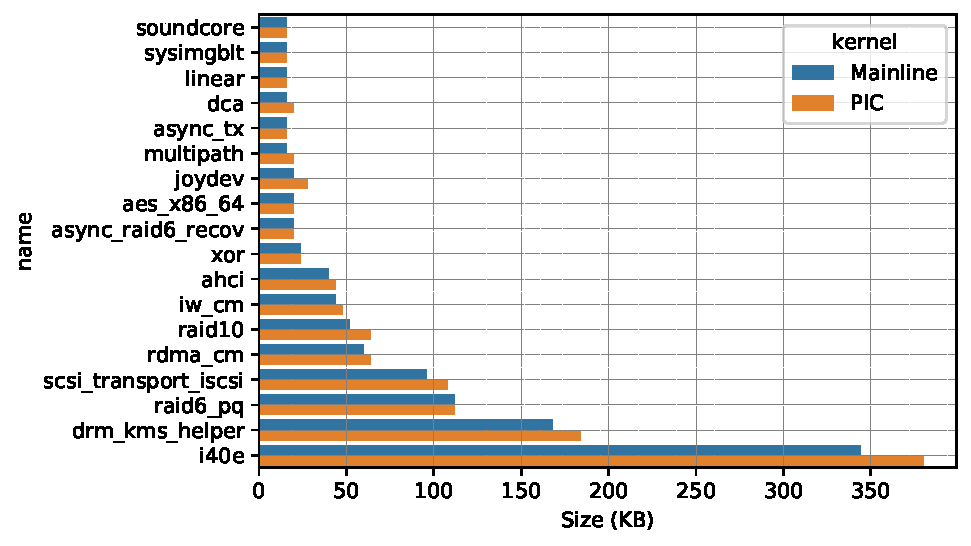
\includegraphics[width=0.7\columnwidth]{charts/module_sizes.pdf}
\caption{Module size (PIC vs. non-PIC), KB}
\label{fig:modulesiszes}
\end{figure}

We first conducted various experiments to test position-independent modules (our first contribution), their overall impact on system performance, and memory footprint.

In Figure~\ref{fig:modulesiszes}, we randomly selected twenty modules to demonstrate the difference in memory footprint resulting from position-independent (PIC) model.
We found the difference in memory footprint of retpoline and non-retpoline cases to be insignificant; thus, we only present the position-independent and the mainline Linux modules with retpoline enabled. Our analysis show that PIC causes an increase in memory footprint of about 10 \%.

Next we ran several micro- and macro- benchmarks to evaluate the performance impact of PIC modules. We evaluated four Linux configurations:
\begin{enumerate}[noitemsep]
    \item Mainline Linux without retpoline
    \item Mainline with retpoline
    \item Our PIC changes without retpoline
    \item Our PIC changes with retpoline
\end{enumerate}
We used the default Ubuntu configuration in all tests. Since we performed some file system tests, we also
compiled the \verb|ext4| Linux filesystem driver as a module.

\begin{figure}[ht!]
\centering
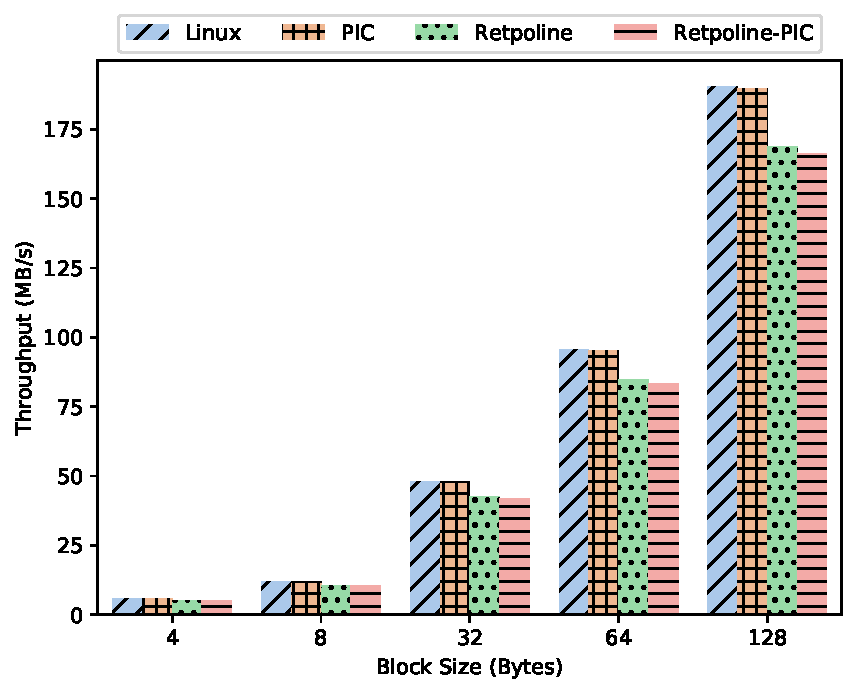
\includegraphics[width=0.7\columnwidth]{charts/file_micro.pdf}
\caption{Filesystem Microbenchmark}
\label{fig:file_micro}
\end{figure}

Figure~\ref{fig:file_micro} shows the results of our own micro-benchmark which uses \verb|dd| to read files with varying block sizes. This test is CPU bound due to the use of the buffer cache. This experiment revealed the real impact of retpoline (Spectre mitigation patches). Figure \ref{fig:file_micro} shows that without retpoline the performance of PIC and non-PIC is nearly the same. There is some performance penalty introduced by the PIC code when retpoline is enabled. This slight performance degradation is caused by the need of \verb|retpoline safe| indirect jumps to external functions in \verb|PLT| stubs of the position independent code.

We used  the \verb|sysbench file_io| benchmark to measure the throughput on random and sequential reads. For this experiment, the files were also cached in RAM to keep the results I/O invariant. The results in Figure~\ref{fig:sysbench_file} show that the performance of PIC-enabled systems is identical to their non-PIC counterparts.

\begin{figure}[ht!]
\centering
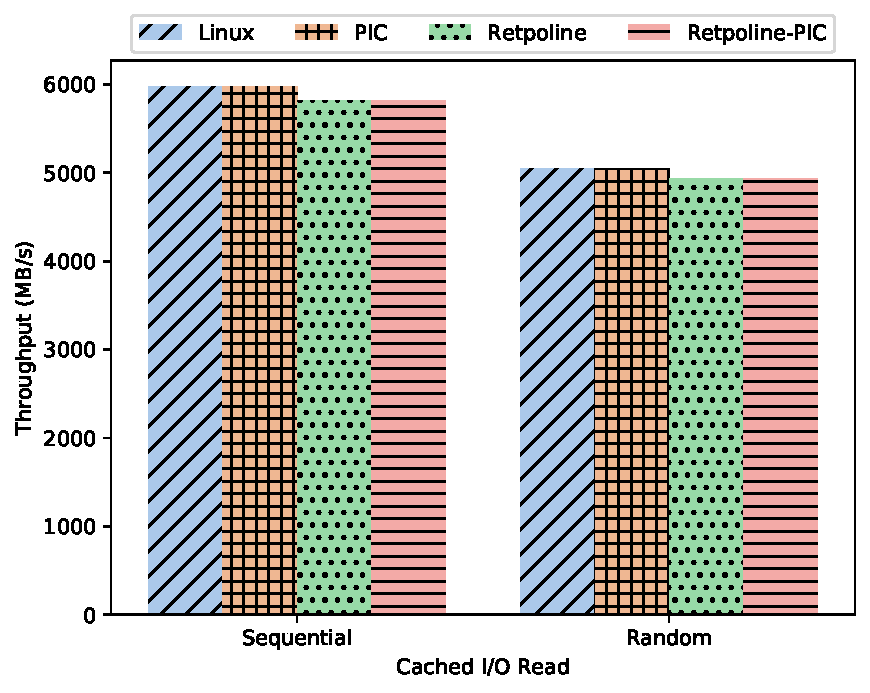
\includegraphics[width=0.7\columnwidth]{charts/sysbench_io.pdf}
\caption{Sysbench Filesystem (Cached)}
\label{fig:sysbench_file}
\end{figure}

\verb|Kernbench| is a CPU throughput benchmark that is often used to compare kernels. We recorded system time (time spent in kernel space) at 3 levels of concurrency. The results as reported in Figure~\ref{fig:kernbench} show that PIC modules have insignificant performance impact.

\begin{figure}[ht!]
\centering
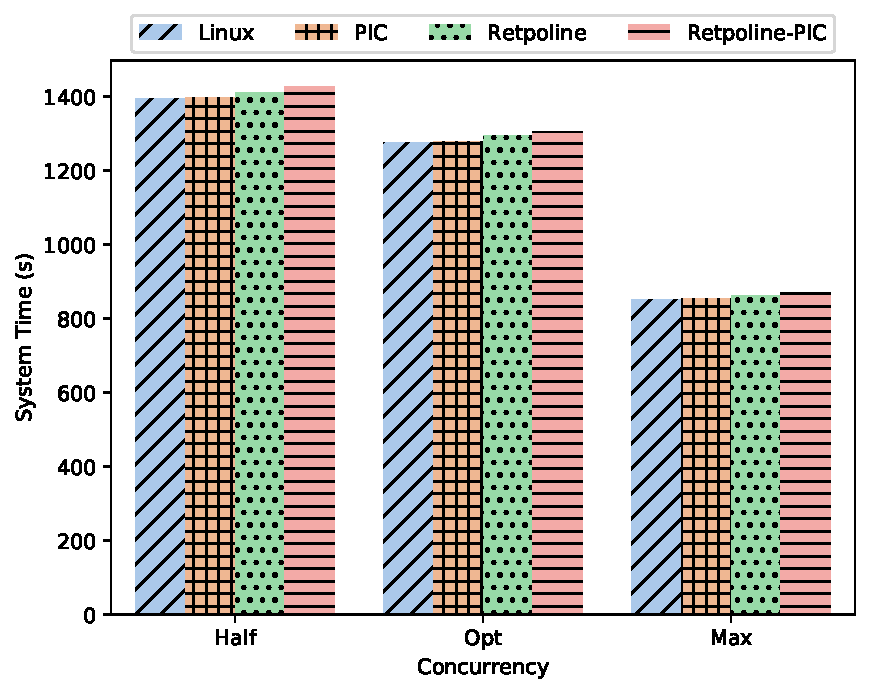
\includegraphics[width=0.7\columnwidth]{charts/kernbench.pdf}
\caption{Kernbench}
\label{fig:kernbench}
\end{figure}

Our tests show that when retpoline is disabled the PIC code performs just the same as its non-PIC counterpart. In the case when retpoline is enabled, PIC code causes slight performance degradation which is almost negligible. Since the effect of retpoline is insignificant, in the later sections we limit the comparison of our work to mainline Linux compiled with retpoline enabled.

\section{Re-Randomization}
\label{sec:eval:rand}
There is currently no continuous re-randomization solution available for the Linux kernel. Therefore, we compare our implementation directly with vanilla Linux. In this report, we evaluate two classes of randomized drivers. First, we evaluate the \verb|e1000e| network driver, which is a popular Intel's Ethernet driver. Then we evaluate the \verb|NVM Express block device| driver that is used for NVMe solid state drives.

\subsection{Network Driver Re-Randomization}
To evaluate network driver re-randomization, we use Apache and mySQL server installations with default Ubuntu configurations. We ran the corresponding macro-benchmarks from a client machine which is directly connected to the network adapter of our test box (server).

In Figure~\ref{fig:network}, we present results for continuous module re-randomization for different block sizes (512B, 1KB, 4KB and 16KB). Smaller block sizes typically put more stress on the system as the total number of system calls increases. We set different re-randomization intervals (1 and 5 ms) and compare against mainline Linux. We present CPU usage across all CPUs.
As Figure~\ref{fig:network} shows, re-randomization does not impact overall system throughput even for high concurrency. Re-randomization does result is slightly elevated CPU usage ($\approx 2 \%$ for 1 ms); the additional CPU usage is independent of the network load and concurrency.

\begin{figure}[ht!]
\centering
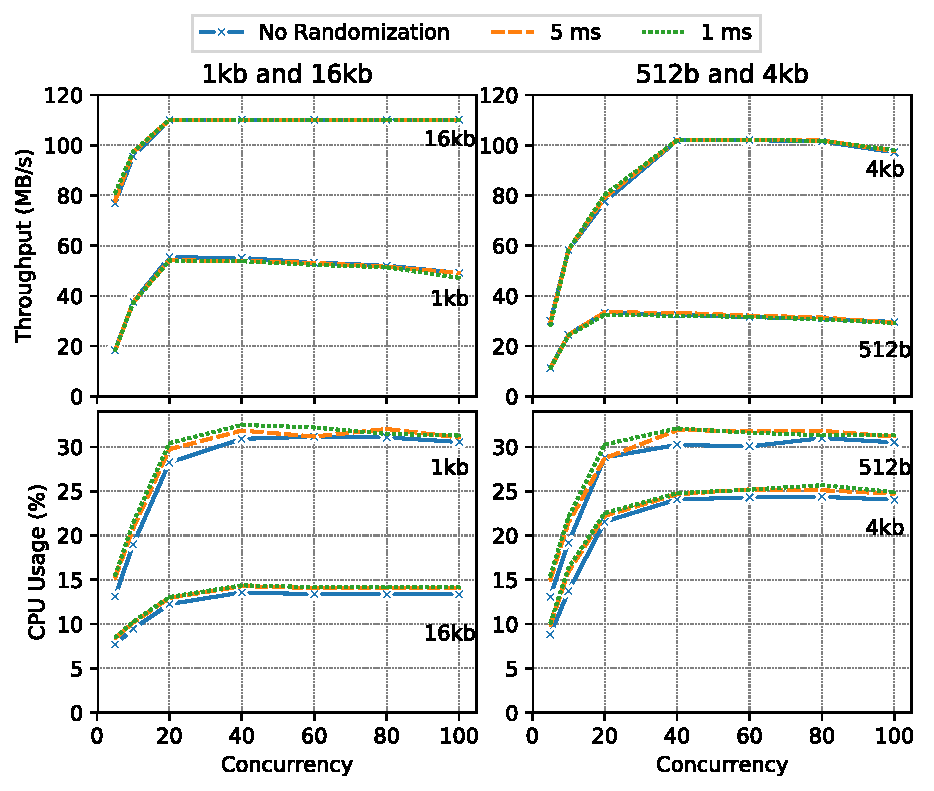
\includegraphics[width=0.8\columnwidth]{charts/apache.pdf}
\caption{ApacheBench: module re-randomization}
\label{fig:network}
\end{figure}

We also measured \verb|mySQL| performance using \verb|sysbench| \verb|oltp| on a database comprising of 10 tables with 1,000,000 rows of data each. The database was cached in memory and the experiment was conducted with varying levels of concurrency and different re-randomization periods. The rate of transactions was measured along with network throughput and CPU utilization, and the results are shown in Figure~\ref{fig:sysbench_sql}. The graphs show that the database performance is unaffected by a re-randomization period and the additional CPU utilization is independent of the system load.

\begin{figure}[ht!]
\centering
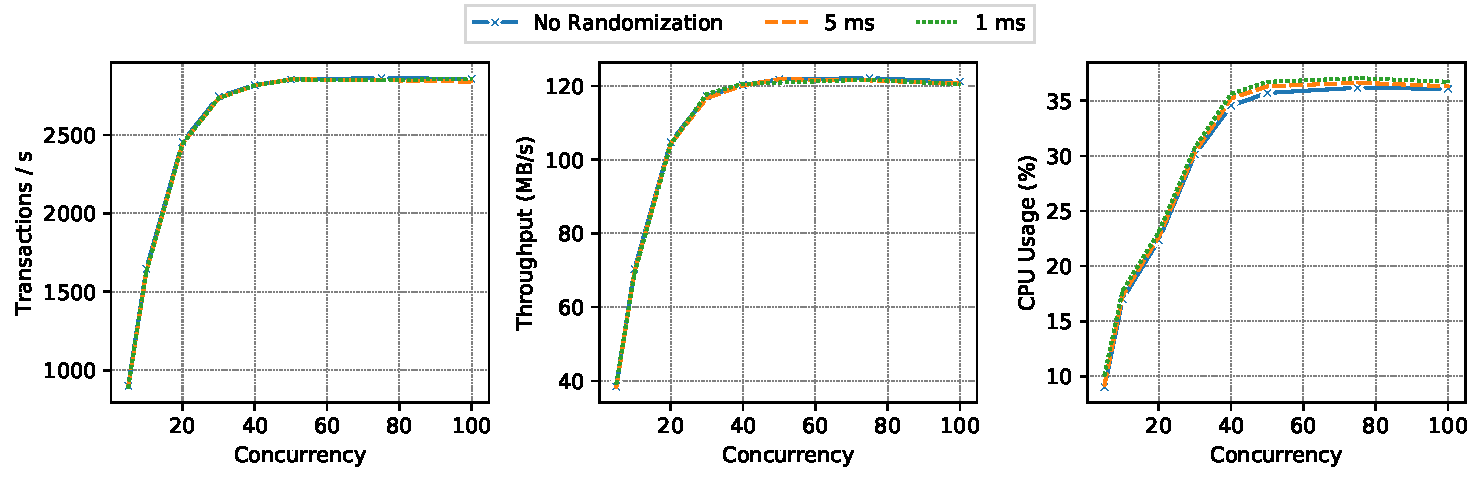
\includegraphics[width=\columnwidth]{charts/sysbench_sql.pdf}
\caption{Sysbench OLTP}
\label{fig:sysbench_sql}
\end{figure}

\subsection{NVMe Driver Re-Randomization}
In order to reliably measure the performance of the NVMe driver under re-randomization, it was important to design an experiment that minimizes the effects of I/O in the underlying hardware. We created our own benchmark that measures the read throughput of a file stored on the NVMe storage. The file is opened with \verb|O_DIRECT| and \verb|O_SYNC| flags using the \verb|open()| syscall, and a block (of 512 bytes) is repeatedly read from the start of the file in a tight loop. The \verb|O_DIRECT| and \verb|O_SYNC| flags guarantee synchronous data transfer and thus prevent caching of the file by the file-system. We read the same block over and over again to leverage the NVMe's internal DRAM cache in an effort to minimize the I/O wait time and make the benchmark CPU bound.

\begin{figure}[ht!]
\centering
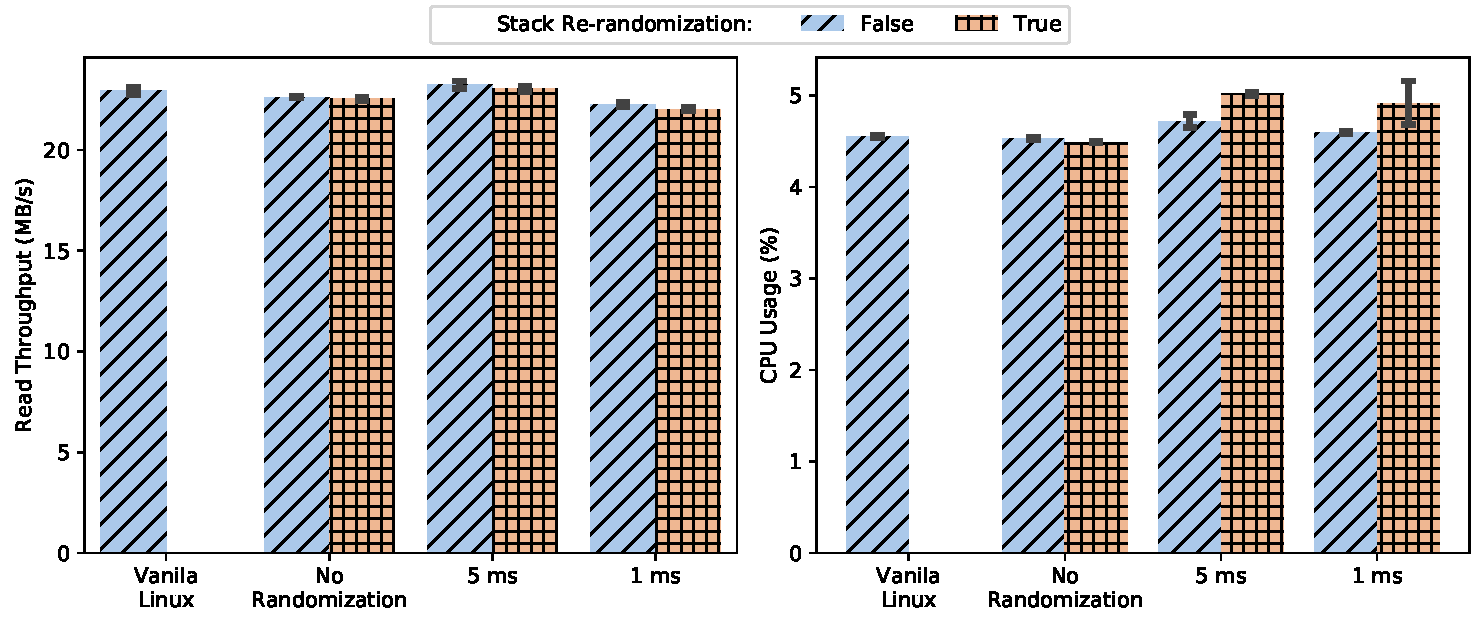
\includegraphics[width=\columnwidth]{charts/nvme_read.pdf}
\caption{NVME Read Throughput}
\label{fig:nvme_read}
\end{figure}

We measured the read throughput of the NVMe drive and recorded the CPU utilization for the duration of the experiment. The results are shown in Figure~\ref{fig:nvme_read}. Apart from the slight increase in CPU utilization, the performance of NVMe storage remains largely unaffected by re-randomization.

\subsection{IOCTL Re-Randomization}
All of our experiments on real-life device drivers showed that re-randomization does not impact the device performance. This can be attributed to the fact that device drivers are I/O bound. The I/O wait time of the device drivers outweighs the CPU time by a large margin and thus the I/O performance penalty due to increased CPU time is minimized. We tested the extreme case of a CPU bounded device driver by designing our own micro-benchmark.

\begin{figure}[ht!]
\centering
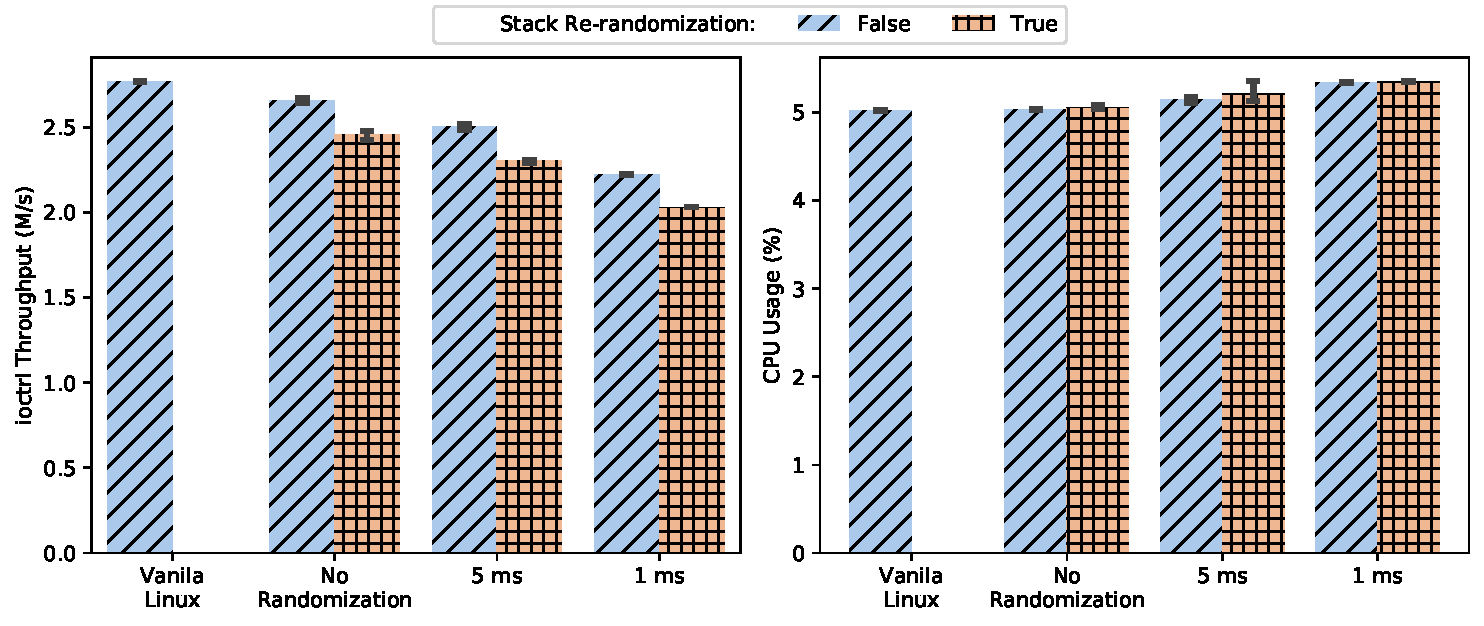
\includegraphics[width=\columnwidth]{charts/ioctrl.pdf}
\caption{IOCTL Throughput}
\label{fig:ioctl}
\end{figure}

We created a dummy device driver that implements a simple \verb|ioctl| operation that just increments the \verb|int| pointer argument passed to it. We repeatedly make the \verb|ioctl()| syscall on the driver in a tight loop and measure the number of ioctl operations performed per second. Figure~\ref{fig:ioctl} shows the ioctl throughput (in million operations per second) along with the corresponding CPU utilization. This benchmark is CPU bound and captures the impact of function wrappers and stack randomization on CPU intensive device operations. It is found that introduction of function wrappers causes a performance drop of $\approx$4\% and stack randomization causes an additional drop of $\approx$6\% when compared to vanilla Linux.

\section{Scalability Analysis}
\begin{wrapfigure}{R}{0.5\columnwidth}
\caption{Re-Randomization Breakdown}
\label{fig:rand_profile}
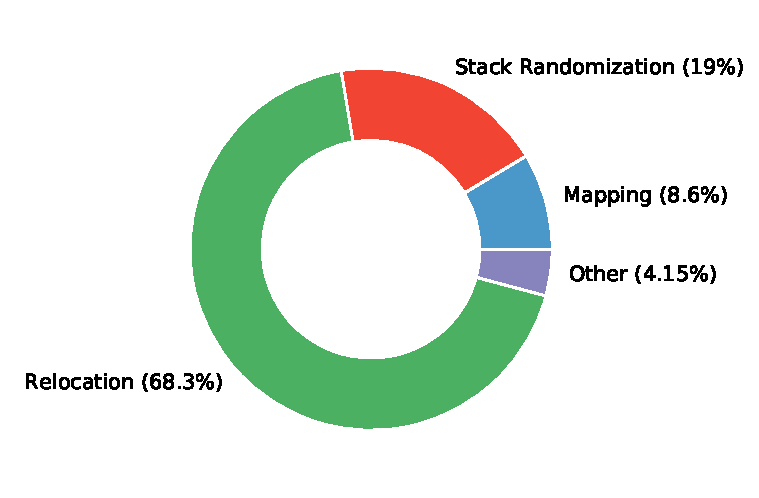
\includegraphics[width=0.5\columnwidth]{charts/rand_profile.pdf}
\end{wrapfigure}

We measured the CPU utilization of the randomization thread to be $0.4\%$ for a randomization period of 20 ms. The breakdown of the CPU utilization is shown in Figure~\ref{fig:rand_profile}. The \textit{stack randomization} and \textit{other} cost is a one-time cost of randomization, independent of the number of modules being randomized. The \textit{virtual page remapping} cost is proportional to the size of the module.

The \textit{relocation} cost is a function of relocation entries in the module object file. Although the re-randomization process only needs to re-apply a fraction of the total relocations in the object file, it has to iterate over all the entries to identify the relevant relocations. We believe with appropriate compiler modifications, the required relocations could be grouped together which would substantially cut down this cost.

A typical server has average utilization of about 20 to 30\%~\cite{bohrer2002case,33387}. With the default Ubuntu configuration, a typical system would use around 100 modules. With 0.32\% CPU utilization per module, our randomization approach can comfortably re-randomize over 150 modules without impacting system performance.

% ============================================================
% ============================================================
% ============================================================

\section{Security Analysis}\label{se:eval_security}
\subsection{Distribution and Availability of ROP gadgets}
In order to gauge the threat posed by ROP gadgets in Linux kernel and to determine the efficacy of our re-randomization approach we used the metrics provided by Follner, et al.~\cite{follner2016analyzing}. We measure the quantity and quality of gadgets in the Linux kernel and its modules. We used Ropper~\cite{schirra_2019}, an ROP gadget finding tool. Ropper can read ELF files, find ROP gadgets and build chains. We studied the ROP gadgets present in Ubuntu 18.04 with default configuration classified under the following three classes:

\begin{enumerate}[noitemsep]
    \item Core Linux kernel
    \item Vanilla modules
    \item PIC modules
\end{enumerate}

Follner, et al.~\cite{follner2016analyzing} proposes two metrics to measure the quantity and quality of ROP gadgets. The first metric is calculated by counting the number of gadgets belonging to twelve proposed categories of operations (Table~\ref{tbl:gadget_categories}). This metric provides information on the quantity of gadgets and is helpful in comparing the number of gadgets between transformed binaries (for example regular modules and PIC modules). The second metric assigns a quality score to an ROP chain based on pre-conditions and side-effects on other registers or memory that a gadget in the chain might have. In our analysis we measure the first metric exactly as proposed by Follner. However, we employ a simplified version of the second metric: we only track if an ROP chain can be constructed with/without side-effects or not.

\newcolumntype{L}{>{\raggedright\arraybackslash}m{12cm}}
\begin{table*}
    \caption{Gadget Categories}
    \begin{center}
    \begin{tabular}{lL}
    \toprule
    \textbf{Category} & \textbf{Included Instructions} \\
    \midrule
    Data move & pop, push, mov, xchg, lea, cmov, movabs \\
    \hline
    Arithmetic & add, sub, inc, dec, sbb, adc, mul, div, imul, idiv, xor, neg, not \\
    \hline
    Logic & cmp, and, or, test \\
    \hline
    Control flow & call, sysenter, enter, int, jmp, je, jne, jo, jp, js, lcall, ljmp, jg, jge, ja, jae, jb, jbe, jl, jle, jno, jnp, jns, loop, jrcxz \\
    \hline
    Shift \& Rotate & shl, shr, sar, sal, ror, rol, rcr, rcl \\
    \hline
    Setting flags & xlatb, std, stc, lahf, cwde, cmc, cld, clc, cdq \\
    \hline
    String & stosd, stosb, scas, salc, sahf, lods, movs \\
    \hline
    Floating point & divps, mulps, movups, movaps, addps, rcpss, sqrtss, maxps, minps, andps, orps, xorps, cmpps, vsubpd, vpsubsb, vmulss, vminsd, ucomiss, subss, subps, subsd, divss, addss, addsd, cvtpi2ps, cvtps2pd, cvtsd2ss, cvtsi2sd, cvtsi2ss, cvtss2sd, mulsd, mulss, fmul, fdiv, fcomp, fadd \\
    \hline
    Misc & wait, set, leave \\
    \hline
    MMX & pxor, movd, movq \\
    \hline
    NOP & nop \\
    \hline
    RET & ret \\
    \bottomrule
    \end{tabular}
    \end{center}
    \label{tbl:gadget_categories}
\end{table*}


\subsubsection*{Gadget Quantity}
The gadget distribution (first) metric measures the number of gadgets falling into twelve broad categories. Each of these categories representing a broad class of operations such as arithmetic, logic etc, as tabulated in Table~\ref{tbl:gadget_categories}. This metric ``allows comparing whether the distribution of gadgets in a transformed binary is similar to the one in original binary, or if the number of gadgets in a category useful for an attacker has grown"~\cite{follner2016analyzing}.

We measure the number of gadgets found for each of these twelve categories of operations. Gadget category is assigned based on the first instruction in the gadget and we only consider gadgets containing six or less instructions. The results are tabulated in Table~\ref{tbl:gadget_quantity} and the same data is visualized as a stacked bar chart in Figure~\ref{fig:gadget_dist}.


\begin{table*}
    \caption{Gadget Quantity for default Ubuntu configuration}
    \begin{center}
    \begin{tabular}{l|l|l|l}
    \toprule
    \textbf{Category} & Kernel & Modules & PIC Modules \\
    \toprule
    Data move & 81489 & 399461 & 539872  \\
    \hline
    Arithmetic & 96201 & 519097 & 649101 \\
    \hline
    Logic & 40241 & 117685 & 192249 \\
    \hline
    Control flow & 44421 & 151590 & 267322 \\
    \hline
    Shift \& Rotate & 13789 & 50598 & 51645  \\
    \hline
    Setting flags & 5137 & 12911 & 91534  \\
    \hline
    String & 973 & 887 & 938 \\
    \hline
    Floating point & 1209 & 5734 & 5745 \\
    \hline
    Misc & 1066 & 4107 & 4788 \\
    \hline
    MMX & 13 & 210 & 208 \\
    \hline
    NOP & 1317 & 3575 & 191057 \\
    \hline
    RET & 11213 & 81237 & 78084 \\
    \bottomrule
    \end{tabular}
    \end{center}
    \label{tbl:gadget_quantity}
\end{table*}

As can be seen in Figure~\ref{fig:gadget_dist}, most of the gadgets are found in the modules, and the core kernel makes up only a tiny proportion of the total gadgets. This validates our work -- re-randomization of just the modules could bring the total number of available gadgets down by about 85 \%.

Kernel modules compiled as position independent code (PIC) is a prerequisite for re-~randomization. Figure~\ref{fig:gadget_dist} shows how compiling the kernel modules as PIC affects the availability of gadgets in the kernel. PIC modules cause a sizable increase in the number of gadgets. This can be attributed to increase in code size. There is an overhead associated with position independent code. With PIC, global data is accessed through GOT, so often additional code is needed to read data from the GOT. Similarly, non-static function calls are made through PLT. All of these indirections result in additional code.
This issue is exacerbated in the recent versions of the Linux kernel that contain Meltdown and Spectre bug fixes. The bug fixes introduce retpolines. A retpoline is a code trampoline (more code!) that prevents the CPU from speculating on the target of an indirect jump. Since PIC increases the occurrences of indirect jumps, the number of retpoline increases resulting in more code, hence the increase in gadget count is expected.

It is important to note that even though PIC causes an increase in the total number of gadgets, the number of gadgets is inconsequential when re-randomization is enabled as these gadgets would not be available to build ROP chains.

\begin{figure}[ht!]
\centering
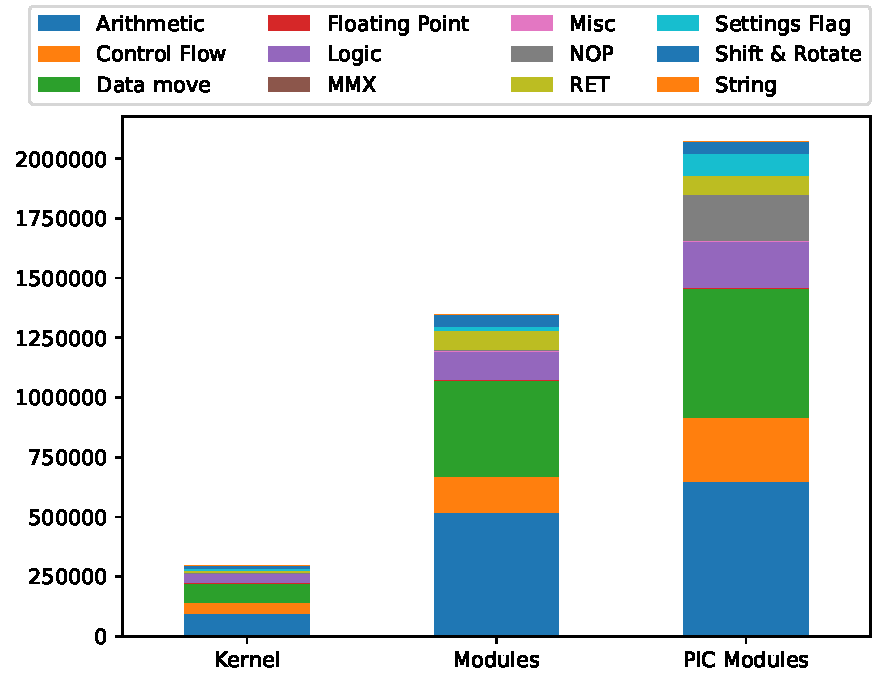
\includegraphics[width=0.6\columnwidth]{charts/gadget_distribution.pdf}
\caption{ROP Gadget Distribution}
\label{fig:gadget_dist}
\end{figure}

\subsubsection*{Gadget Quality}
To evaluate the quality of gadgets (second metric), we need to consider a concrete goal that an attacker might be interested in achieving. In our analysis, we consider the
\begin{lstlisting}
set_memory_x(unsigned long addr, int numpages)
\end{lstlisting}
function. This function is an attractive target for an attacker because by calling this function with appropriate arguments an attacker could disable the no-execute (NX) protection on memory pages of his choice. After disabling NX protection, any arbitrary code can be executed from target memory. In order to construct an ROP chain to disable the NX protection, the attacker first begins by targeting a particular memory address and then prepares the environment and function arguments. The ROP chain needs to contain instructions to perform the following operations:
\begin{enumerate}[noitemsep]
    \item Pivor Stack
    \item Load \verb|addr| argument into the register \verb|RDI|
    \item Load \verb|num_pages| argument into register \verb|RSI|
    \item Call \verb|set_memory_x|
\end{enumerate}

For all the available modules, we try to construct an ROP gadget to call the \verb|set_memory_x| function. Furthermore, we track if the ROP gadget has side-effects. The results are shown in Table~\ref{tbl:gadget_quality}. 80\% of the modules contain enough gadgets to form a ROP chain to disable NX protection.

\begin{table*}
    \caption{Gadget Categories}
    \begin{center}
    \begin{tabular}{lcc}
    \toprule
     & \textbf{Non-PIC} & \textbf{PIC} \\
    \midrule
    \textbf{Modules with ROP Chain, no side-effect} & 4,320 & 4,358 \\
    \textbf{Modules with ROP Chain, with side-effect} & 1 & 1 \\
    \textbf{Modules without ROP Chain} & 1,008 & 970 \\
    \hline
    \textbf{Total Number of Modules} & 5,329 & 5,329 \\
    \bottomrule
    \end{tabular}
    \end{center}
    \label{tbl:gadget_quality}
\end{table*}

From our evaluation, we found that Linux kernel modules contain 85\% of all the available gadgets. And 80\% of the modules contain enough gadgets to disable the NX protection without any side effects. Hence, re-randomization of the modules is a promising approach to mitigating the ROP attacks on Linux kernel.
	\chapter{Conclusions and Future Work} \label{ch:conclusion}
        In this thesis, we presented a technique to prevent code-reuse attacks on the Linux kernel modules. We added support for position-independent code model and demonstrated the first-ever implementation of code re-randomization for the Linux kernel modules. Both of these contributions increase the entropy and reduce the chances of a successful ROP attack. Our experiments show that our implementation results in a negligible effect on system performance.

\section{Conclusions}
As discussed in Section~\ref{sec:bg_rop}, \textit{executable space protection} is a computer security technique of marking memory regions as non-executable. The widespread adoption of this technique has virtually eliminated \textit{code injection} attacks on modern systems. Code injection, which was once one of the most important techniques used by attackers to gain unauthorized access to the system, has been replaced by \textit{code reuse attacks}. Code reuse attacks exemplified by \textit{return oriented programming (ROP)} reuse fragments of existing code to perform arbitrary actions and thus avoid the need for injecting code.

\textit{Kernel address-space layout randomization (KASLR)} is a security technique currently employed by the Linux kernel to make successful ROP attacks harder to launch. With KASLR, the kernel and its modules are loaded at random addresses at boot time. This defense is a ``statistical defense" since it is based on the chances of the attacker guessing the random load address. The effectiveness of KASLR is thus proportional to the entropy of the random offset. It turns out that the current implementation of KASLR is severely limited in this randomness as the kernel modules can only be loaded within a 1GB range of the kernel image. Additionally, KASLR is further undermined by the presence of memory disclosure vulnerabilities. Memory leakages can be used to discover code gadgets at runtime in a technique known as \textit{Just-In-Time ROP (JIT-ROP)}.

In this thesis, we contributed towards kernel hardening by increasing the entropy of KASLR randomization and designing a code re-randomization technique for the Linux kernel. In Chapter~\ref{ch:pic} we discussed our implementation of position independent model (PIC) for the kernel modules. This contribution is submitted to  one of the Linux kernel hardening mailing lists and is currently under review~\cite{pie_patch_1:online,pie_patch_2:online}. Position independent kernel modules can be loaded anywhere in the 64-bit address space and makes guessing the base address of the module almost impossible.

The second major contribution of this thesis is the continuous re-randomization of kernel modules. We have described our implementation in detail in Chapter~\ref{ch:re_randomization}. Unlike existing user-space solutions, our technique uses a zero-copying method for moving data and code, and efficiently keeps track of and unmaps previously used address ranges. We are able to randomize a module and its stack at very high randomization frequencies (< 1ms) without significant performance degradation.

This is the first re-randomization implementation in kernel space. Kernel space creates additional challenges due to a low-level API, involving system calls, interrupt handling, and hardware access in device drivers. A code change at the operating system level has the potential to affect all the user space applications. We were thus very mindful of performance in our design. Our implementation is highly efficient with very little overhead (< 2\%) for re-randomization and completely negligible overhead for supporting extended KASLR with position-independent modules as compared to the vanilla Linux. We have evaluated our work in great detail in Chapter~\ref{ch:evaluation}.

Our re-randomization technique is highly efficient. The low overhead of our re-randomization thread and insignificant performance degradation of the randomized module is largely thanks to our \textit{zero-copy} approach. With the \textit{zero-copy} approach, the re-randomization thread only needs to create a new virtual address mapping instead of duplicating the memory pages, and since both the old and new address spaces remain mapped during the re-randomization process, the re-randomized module does not need to be paused for re-randomization. We believe this low overhead would help widespread adoption of our re-randomization technique.

\section{Future Work}
This thesis is the first effort to implement a re-randomization solution for kernel space and opens new avenues for further development in this area:

% Our work focused on the re-randomization of just the kernel modules. It was argued that by compiling most of the kernel as modules, the core kernel image can be reduced to a bare minimum. The small code base of the core kernel can be trusted to not have any bugs that leak memory. Without memory disclosure vulnerabilities in the core kernel, it is safe from JIT-ROP attacks. Our first proposal for future work is to reduce the trusted code base even further by having the kernel run on top of a thin hypervisor. The interface between a paravirtualized guest kernel and the hypervisor is similar to the interface between a kernel and a module. Our re-randomization technique could be extended to support re-randomization of the kernel running on a hypervisor.

We demonstrated our re-randomization technique by manually modifying the source code of the modules to support re-randomization. Making a module re-randomization friendly involves wrapping the interface between the kernel and the module. We propose a compiler plugin to identify and wrap all the functions and variables in the module that are exposed to the kernel. Linux kernel has more than 5000 modules, manually modifying the modules to be re-randomizable is not practical. Implementation of a compiler plugin to automate this process is paramount to reap the benefits of re-randomization.

Our work re-randomizes the kernel modules and the core kernel is left un-randomized. A randomized module is still capable of leaking a pointer to the core kernel. This is a security risk as the attacker can now harvest the code pages in the (un-randomized) core kernel and it might be possible to construct a JIT-ROP gadget consisting of the code from the core kernel alone. This can be prevented by encrypting the kernel references in the module. Pointers to the kernel can reside in the code or on the stack, both of which are already wrapped by our code and it is possible to add the encryption/decryption in the already existing wrappers. We leave the encryption of kernel pointers as a work for the future.

Our re-randomization technique provides limited support for \textit{global variable code pointers}. The value of a variable code pointer is evaluated at run-time. Since we do not unmap the old address space while a module function is under execution, a \textit{local variable pointer} reference never breaks, a global variable pointer can however break and must be handled uniquely during re-randomization. In contrast, a \textit{constant code pointer's} value is known at compilation time and there exists a corresponding relocation entry in the relocation table. In our implementation, we update all const pointers using the relocation table but a variable pointer must be handled differently. A naive approach is to \textit{wrap} all the functions referenced by the variable code pointers since function wrappers are not re-randomized, the pointers will remain valid after re-randomization. This approach introduces indirection to local function calls, can cause performance impact and hence may not be practical. In our research, none of the modules we worked with so far used variable global pointers, but such modules may exist. It is proposed that alternative techniques such as pointer tracking be explored to handle such cases.

	\bibliography{bibliography,bib_ruslan}
	\bibliographystyle{plainnat}

\end{document}


%****************************************************************************
% Below are some general suggestions for writing your dissertation:
%
% 1. Label everything with a meaningful prefix so that you
%    can refer back to sections, tables, figures, equations, etc.
%    Usage \label{<prefix>:<label_name>} where some suggested
%    prefixes are:
%			ch: Chapter
%     		se: Section
%     		ss: Subsection
%     		sss: Sub-subsection
%			app: Appendix
%     		ase: Appendix section
%     		tab: Tables
%     		fig: Figures
%     		sfig: Sub-figures
%     		eq: Equations
%
% 2. The VTthesis class provides for natbib citations. You should upload
%	 one or more *.bib bibtex files. Suppose you have two bib files: some_refs.bib and 
%    other_refs.bib.  Then your bibliography line to include them
%    will be:
%      \bibliography{some_refs, other_refs}
%    where multiple files are separated by commas. In the body of 
%    your work, you can cite your references using natbib citations.
%    Examples:
%      Citation                     Output
%      -------------------------------------------------------
%      \cite{doe_title_2016}        [18]
%      \citet{doe_title_2016}       Doe et al. [18]
%      \citet*{doe_title_2016}      Doe, Jones, and Smith [18]
%
%    For a complete list of options, see
%      https://www.ctan.org/pkg/natbib?lang=en
%
% 3. Here is a sample table. Notice that the caption is centered at the top. Also
%    notice that we use booktabs formatting. You should not use vertical lines
%    in your tables.
% 
%				\begin{table}[htb]
%					\centering
%					\caption{Approximate computation times in hh:mm:ss for full order 						versus reduced order models.}
%					\begin{tabular}{ccc}
%						\toprule
%						& \multicolumn{2}{c}{Computation Time}\\
%						\cmidrule(r){2-3}
%						$\overline{U}_{in}$ m/s & Full Model & ROM \\
%						\midrule
%						0.90 & 2:00:00 & 2:08:00\\
%						0.88 & 2:00:00 & 0:00:03\\
%						0.92 & 2:00:00 & 0:00:03\\
%						\midrule
%						Total & 6:00:00 & 2:08:06\\
%						\bottomrule
%					\end{tabular}
%					\label{tab:time_rom}
%				\end{table}
% 
% 4. Below are some sample figures. Notice the caption is centered below the
%    figure.
%    a. Single centered figure:
%					\begin{figure}[htb]
%						\centering
%						\includegraphics[scale=0.5]{my_figure.eps}
%						\caption{Average outlet velocity magnitude given an average  
%				        input velocity magnitude of 0.88 m/s.} 
%						\label{fig:output_rom}
%					\end{figure}
%    b. Two by two grid of figures with subcaptions
%					\begin{figure}[htb]
%						\centering
%						\begin{subfigure}[h]{0.45\textwidth}
%							\centering
%							\includegraphics[scale=0.4]{figure_1_1.eps}
%							\caption{Subcaption number one}
%							\label{sfig:first_subfig}
%						\end{subfigure}
%						\begin{subfigure}[h]{0.45\textwidth}
%							\centering
%							\includegraphics[scale=0.4]{figure_1_2.png}
%							\caption{Subcaption number two}
%							\label{sfig:second_subfig}
%						\end{subfigure}
%
%						\begin{subfigure}[h]{0.45\textwidth}
%							\centering
%							\includegraphics[scale=0.4]{figure_2_1.pdf}
%							\caption{Subcaption number three}
%							\label{sfig:third_subfig}
%						\end{subfigure}
%						\begin{subfigure}[h]{0.45\textwidth}
%							\centering
%							\includegraphics[scale=0.4]{figure_2_2.eps}
%							\caption{Subcaption number four}
%							\label{sfig:fourth_subfig}
%						\end{subfigure}
%						\caption{Here is my main caption describing the relationship 							between the 4 subimages}
%						\label{fig:main_figure}
%					\end{figure}
%
%----------------------------------------------------------------------------
%
% The following is a list of definitions and packages provided by VTthesis:
%
% A. The following packages are provided by the VTthesis class:
%      amsmath, amsthm, amssymb, enumerate, natbib, hyperref, graphicx, 
%      tikz (with shapes and arrows libraries), caption, subcaption,
%      listings, verbatim
%
% B. The following theorem environments are defined by VTthesis:
%      theorem, proposition, lemma, corollary, conjecture
% 
% C. The following definition environments are defined by VTthesis:
%      definition, example, remark, algorithm
%
%****************************************************************************